\documentclass[12pt,a4paper]{article}

\usepackage[utf8]{inputenc}
\usepackage[T1]{fontenc}
\usepackage[english]{babel}
\usepackage{geometry}
\geometry{a4paper, top=2.5cm, bottom=2.5cm, left=2.5cm, right=2.5cm}
\usepackage{graphicx}
\usepackage{hyperref}
\usepackage{booktabs}
\usepackage{enumitem}
\usepackage{listings}
\usepackage{xcolor}
\usepackage{float}
\usepackage{pdflscape}
\usepackage{caption}
\usepackage{amsmath}
\usepackage{amssymb}
\usepackage{hyperref}
\usepackage{listings}
\graphicspath{{img/}}

\lstset{
    language=SQL,
    basicstyle=\ttfamily\small,
    keywordstyle=\color{blue}\bfseries,
    stringstyle=\color{red!70!black},
    commentstyle=\color{green!50!black},
    numbers=left,
    numberstyle=\tiny\color{gray},
    stepnumber=1,
    backgroundcolor=\color{gray!5},
    frame=single,
    rulecolor=\color{gray!40},
    breaklines=true,
    captionpos=b,
    showstringspaces=false
}

\hypersetup{
    colorlinks=true,
    linkcolor=black,
    filecolor=magenta,      
    urlcolor=blue,
    pdftitle={smarthealth-db-report},
}

\title{
    \vspace{-2cm}
    
\includegraphics[width=0.5\textwidth]{YTU-Logo.png} \\ 
    \vspace{2cm}
    \Huge \textbf{Smart Healthcare Management} \\
    \vspace{0.5cm}
    \Large Data Management and File Structures 1 Homework Report
}
\author{
    \textbf{Prepared By:} \\ 
    Riza Can Tay \\[0.8cm]
    \textbf{Submitted To:} \\ 
    Prof. Dr. İbrahim Emiroglu\\[1cm]
    \textit{Yildiz Technical University - Department of Mathematical Engineering}
}\date{\vspace{1cm} \today}

\begin{document}

\maketitle
\thispagestyle{empty}
\newpage

\tableofcontents
\newpage

\section{Requirements Analysis}
\label{sec:requirements}

This project, an assignment for the MTM2522 Data Management and File Structures 1 course in the Department of Mathematical Engineering at Yildiz Technical University, is a central database system designed to digitize some basic daily operations of a large hospital network consisting of multiple hospitals. These operations include outpatient appointments, simple doctor-patient interactions, patient records, personnel management, appointment tracking, and financial billing. Pharmacy inventory tracking, hospital inpatient wards (operating rooms, etc.), and many other modules are excluded from the conceptual scope of this project.

\subsection{Entities}

Below is a list of the entities that form the basis of the system, their attributes, and key structures (PK, FK, UNIQUE):

\begin{itemize}[label=\textbf{--}]


	\item \textbf{Person (Superclass):} Contains basic information of all persons registered.
	      \begin{itemize}[label=$\bullet$]
		      \item \texttt{Person\_ID} (PK): Unique primary key automatically assigned to each individual.
		      \item \texttt{National\_ID} (UNIQUE): Person's official national identification number.
		      \item \texttt{Name} (Composite Attribute): Person's name information.
		            \begin{itemize}[label=$\circ$]
			            \item \texttt{First\_Name}: Person's first name information.
			            \item \texttt{Last\_Name}: Person's last name information.
		            \end{itemize}
		      \item \texttt{Date\_of\_Birth}: Person's date of birth.
		      \item \texttt{Gender}, \texttt{Blood\_Type}: Person's gender and blood type information.
		      \item \texttt{Phone\_Number}: Person's contact number.
		      \item \texttt{Address} (Composite Attribute): Person's physical address information.
		            \begin{itemize}[label=$\circ$]
			            \item \texttt{Country}: Country of residence.
			            \item \texttt{City}: City of residence.
			            \item \texttt{District}: District or borough information.
			            \item \texttt{Street}: Street name of the address.
			            \item \texttt{Building\_No}: Building number of the residence.
			            \item \texttt{Apartment\_No}: Apartment number of the residence.
			            \item \texttt{Zip\_Code}: Postal/ZIP code of the address.
		            \end{itemize}
		      \item \texttt{Email} (UNIQUE), \texttt{Password\_Hash}: Unique email address and encrypted password are used for secure system login.
	      \end{itemize}

	\item \textbf{Medical\_Staff (Intermediate Superclass):} Groups the personnel authorized to perform medical interventions and inherits from \texttt{Person}.
	      \begin{itemize}[label=$\bullet$]
		      \item \texttt{Person\_ID} (PK): Primary key that references the \texttt{Person} table.
		      \item \texttt{Department\_ID} : Reference from the department the employee belongs to.
	      \end{itemize}

	\item \textbf{Patient (Subclass):} Represents individuals receiving medical services from the hospital and inherits from \texttt{Person}.
	      \begin{itemize}[label=$\bullet$]
		      \item \texttt{Person\_ID} (PK): Primary key that references the \texttt{Person} table.
		      \item \texttt{Allergies} (Multivalued): Reactions by patient's immune system to substances.
	      \end{itemize}

	\item \textbf{Doctor (Medical Subclass):} Represents doctors authorized to provide medical diagnosis and treatment and inherits from \texttt{Medical\_Staff}.
	      \begin{itemize}[label=$\bullet$]
		      \item \texttt{Person\_ID} (PK): Primary key that references the \texttt{Person} table.
		      \item \texttt{Specialty}: Doctor's area of expertise.
		      \item \texttt{License\_Number} (UNIQUE): Doctor's official license number.
		      \item \texttt{Treatments} (Multivalued): Medical methods that doctor has been trained to use to cure patient.
	      \end{itemize}

	\item \textbf{Nurse (Medical Subclass):} Represents nurses working in the hospital and inherits from \texttt{Medical\_Staff}.

	      \begin{itemize}[label=$\bullet$]
		      \item \texttt{Person\_ID} (PK): Primary key that references the \texttt{Person} table.
	      \end{itemize}

	\item \textbf{Admin (Subclass):} Represents the senior staff responsible for the administration and inherits from \texttt{Person}.
	      \begin{itemize}[label=$\bullet$]
		      \item \texttt{Person\_ID} (PK): Primary key that references the \texttt{Person} table.
		      \item \texttt{Role\_Level}: Administrator's level of authority.
		      \item \texttt{MFA\_Secret} (NOT NULL): Security key used for two-factor authentication.
	      \end{itemize}

	\item \textbf{Staff (Subclass):} Represents non-medical support staff (cleaning, security, consulting, etc.) and inherits from \texttt{Person}.
	      \begin{itemize}[label=$\bullet$]
		      \item \texttt{Person\_ID} (PK): Primary key that references the \texttt{Person} table.
		      \item \texttt{Job\_Title}: Job description of the staff.
	      \end{itemize}

	\item \textbf{Disease:} Refers to process of identifying a disease or condition
	      \begin{itemize}[label=$\bullet$]
		      \item \texttt{Disease\_ID} (PK): Unique registration number assigned to this disease by system.
		      \item \texttt{Disease\_Name}: General name of disease.
		      \item \texttt{Disease\_Type}: General classification of disease (e.g., Chronic, Acute, Infectious).
		      \item \texttt{Symptoms (Multivalued):} Set of symptoms associated with this disease (e.g., shortness of breath, high fever).
	      \end{itemize}

	\item \textbf{Hospital:} Defines physical and organizational data of hospital buildings.
	      \begin{itemize}[label=$\bullet$]
		      \item \texttt{Hospital\_ID} (PK): Hospital's unique code.
		      \item \texttt{Hospital\_Name}: Official name of hospital.
		      \item \texttt{Address} (Composite Attribute): Hospital's address information.
		            \begin{itemize}[label=$\circ$]
			            \item \texttt{Country}: Country where hospital is located.
			            \item \texttt{City}: City where hospital is located.
			            \item \texttt{District}: District or borough of hospital.
			            \item \texttt{Street}: Street name of hospital address.
			            \item \texttt{Building\_No}: Building number of hospital.
			            \item \texttt{Zip\_Code}: Postal/ZIP code of hospital address.
		            \end{itemize}
		      \item \texttt{Contact\_Number}: Contact number of hospital.
	      \end{itemize}

	\item \textbf{Department:} Defines medical or administrative departments operating within hospital.
	      \begin{itemize}[label=$\bullet$]
		      \item \texttt{Department\_ID} (PK): Unique registration number of department.
		      \item \texttt{Hospital\_ID} : Hospital's unique code.
		      \item \texttt{Department\_Name}: Name of the department (Cardiology, Neurology, etc.).
		      \item \texttt{Extension\_Number}: Internal phone number that provides direct access to department.
	      \end{itemize}

	\item \textbf{Room (Weak Entity):} Defines physical rooms within hospital departments and is directly dependent on \texttt{Department} to exist.
	      \begin{itemize}[label=$\bullet$]
		      \item \texttt{Department\_ID} (PK): Unique registration number of department.
		      \item \texttt{Room\_Number} (Partial Key): Door number within department and combines with \texttt{Department\_ID} to form a composite primary key.
		      \item \texttt{Room\_Type}: Purpose of room (Examination Room, Laboratory, Polyclinic, etc.).
	      \end{itemize}

	\item \textbf{Appointment (Associative Entity):} Central process table that tracks relationship between doctor and patient.
	      \begin{itemize}[label=$\bullet$]
		      \item \texttt{Appointment\_ID} (PK): Unique registration number of appointment.
		      \item \texttt{Patient\_ID}\textsuperscript{*} , \texttt{Doctor\_ID}\textsuperscript{*} : References identifying parties to appointment.
		      \item \texttt{Appointment\_Date}, \texttt{Appointment\_Time}: Date and time of appointment.
		      \item \texttt{Status\_ID}: Current status of appointment (0: Cancelled 1:Scheduled 2: Completed, etc.).
		      \item \texttt{Chief\_Complaint}: Primary reason for the patient's visit.
	      \end{itemize}

	\item \textbf{Prescription (Weak Entity):} Records prescriptions written for pations as a result of completed appointments.
	      \begin{itemize}[label=$\bullet$]
		      \item \texttt{Appointment\_ID} : Unique registration number of appointment.
		      \item \texttt{Medication\_Name}: Name of prescribed medication.
		      \item \texttt{Dosage}: Dosage of medication to be used.
		      \item \texttt{Instructions}: Doctor's instructions regarding the use of medication.
	      \end{itemize}

	\item \textbf{Lab\_Result:} Records medical tests and their results requested during appointments.
	      \begin{itemize}[label=$\bullet$]
		      \item \texttt{Lab\_ID} (PK): The unique record number of test result.
		      \item \texttt{Appointment\_ID} : Unique registration number of appointment.
		      \item \texttt{Test\_Type}: Type of test performed (Completed Blood Count, MRI, X-ray, etc.).
		      \item \texttt{Result\_Value}: Numerical or textual result of laboratory
		      \item \texttt{Reference\_Range}: Reference range considered healthy for relevant test.
		      \item \texttt{Test\_Date}: Date the test was performed.
	      \end{itemize}

	\item \textbf{Insurance:} Tracks the private or state-supported health insurance policies held by patients. \begin{itemize}[label=$\bullet$] \item \texttt{Insurance\_ID} (PK): Unique number of insurance record.
		      \item \texttt{Patient\_ID}\textsuperscript{*} : Reference of patient to whom the policy belongs.
		      \item \texttt{Provider\_ID} : Reference of insurance provider.
		      \item \texttt{Policy\_Number}: Policy number assigned by insurance provider.
		      \item \texttt{Coverage\_Rate}: Percentage of insurance's coverage of invoice amount (e.g., \%80).
	      \end{itemize}

	\item \textbf{Billing:} Tracks financial payment status resulting from completed services.
	      \begin{itemize}[label=$\bullet$]
		      \item \texttt{Bill\_ID} (PK): Unique registration number of invoice.
		      \item \texttt{Appointment\_ID} : Unique registration number of the appointment.
		      \item \texttt{Total\_Amount}: Total cost of procedures performed.
		      \item \texttt{Patient\_Share}: Net amount the patient must pay after insurance discount.
		      \item \texttt{Payment\_Status}: Current payment status of invoice (0: Pending, 1: Paid, etc.).
	      \end{itemize}

	\item \textbf{Insurance\_Provider:} Represent private insurance companies or government institutions that patient has agreements with.
	      \begin{itemize}[label=$\bullet$]
		      \item \texttt{Provider\_ID} (PK): Unique number assigned to provider by system.
		      \item \texttt{Provider\_Name}: Official name of insurance provider (Allianz, AXA, etc.).
		      \item \texttt{Tax\_Number}: Provider's official tax number.
		      \item \texttt{Provider\_Email}: Provider's official contact email.
	      \end{itemize}

	\item \textbf{Payer (Union):} Representing anyone who can make payment, formed by union of \texttt{Patient} and \texttt{Insurance\_Provider}.
	      \begin{itemize}[label=$\bullet$]
		      \item \texttt{Payer\_ID} (PK): Unique number assigned to provider by system.
		      \item \texttt{Payer\_Type}: Discriminator that indicates whether payer is natural person or legal entity.
	      \end{itemize}

	\item \textbf{Payment:} Tracks individual financial transactions made to settle billing invoice.
	      \begin{itemize}[label=$\bullet$]
		      \item \texttt{Payment\_ID} (PK): Unique registration number of transaction receipt.
		      \item \texttt{Bill\_ID} : Reference to the invoice being paid.
		      \item \texttt{Payer\_ID} : Reference to entity who made payment.
		      \item \texttt{Amount\_Paid}: Exact monetary value transferred in transaction.
		      \item \texttt{Payment\_Date}: Date and time the transaction was completed.
	      \end{itemize}


\end{itemize}
\vspace{0.2cm}
\noindent \footnotesize{\textit{\textbf{* Note:} \texttt{Patient\_ID} and \texttt{Doctor\_ID} external keys  are named aliases to highlight logic and readability. In the physical database model, these fields directly reference \texttt{Person\_ID} fields of the corresponding subclasses.}}
\subsection{Relationships}

The relationships and cardinalitys of the entities are as follows:

\subsubsection*{Hierarchical Relationships / Inheritance (IS-A)}
\begin{itemize}[label=\textbf{--}]

	\item \textbf{Person -- Patient / Admin / Staff:} All system users are inherits from \texttt{Person} entity.
	\item \textbf{Person -- Medical\_Staff -- Doctor / Nurse:} Medical personnel are structured through a multi-level inheritance hierarchy to ensure proper attribute delegation and specialization.
\end{itemize}

\subsubsection*{Functional Relationships (HAS-A)}
\begin{itemize}[label=\textbf{--}]

	\item \textbf{Hospital -- Department (1:N) :} A single hospital structure contains multiple departments. Each department belongs strictly to this main hospital entity.
	\item \textbf{Department -- Medical\_Staff (1:N) :} A department employs multiple medical staff members. To maintain operational integrity, each medical staff member is officially registered to only one primary department.
	\item \textbf{Department -- Room (1:N) :} A department may have multiple rooms, but each room belongs to its own department.
	\item \textbf{Patient -- Appointment (1:N) :} A registered patient can book multiple appointments over time, but each specific appointment record is assigned to exactly one patient.
	\item \textbf{Doctor -- Appointment (1:N) :} A doctor can conduct multiple appointments, but each individual medical encounter is managed by exactly one specific doctor.
	\item \textbf{Appointment -- Prescription (1:1) :} An appointment can generate at most one prescription, which is directly tied to that specific encounter.
	\item \textbf{Appointment -- Lab\_Result (1:N) :} A single appointment can result in multiple laboratory tests or results, all of which are tracked back to the originating encounter.
	\item \textbf{Appointment -- Billing (1:1) :} Each appointment generates exactly one primary billing record for financial tracking.
	\item \textbf{Patient -- Insurance (1:1) :} A patient holds exactly one primary active insurance policy within the system.
	\item \textbf{Insurance\_Provider -- Insurance (1:N) :} A single insurance provider company can issue multiple insurance policies to different patients, but each policy is strictly managed by one provider.
	\item \textbf{Billing -- Payment (1:N) :} A single generated billing invoice can receive multiple separate payments until total amount is settled.
	\item \textbf{Payer -- Payment (1:N) :} A payer entity can make multiple financial payments over time, but each payment transaction is traced back to exactly one payer.
	\item \textbf{Patient -- Doctor (M:N) :} A patient can be treated by multiple doctors and a doctor can treat multiple patients.
	\item \textbf{Patient -- Disease (M:N) :} A patient can be diagnosed with multiple diseases and a single disease can be diagnosed in multiple patients. Associative relationship (\texttt{Diagnosed\_With}) captures specific attributes.
\end{itemize}
\vspace{0.3cm}

\subsection{Constraints}
To preserve data integrity and accurately reflect real-world hospital operations within the database, the following constraints have been defined:

\subsubsection*{Unique Constraints}
Rules enforcing uniqueness to prevent duplicate records and identity conflicts across the database.
\begin{itemize}[label=\textbf{--}]
	\item \textbf{Citizen and Contact Uniqueness:} National identification number (\texttt{National\_ID}) and email address (\texttt{Email}) in \texttt{Person} entity must be globally unique. Single individual cannot be registered multiple times.
	\item \textbf{Professional Identity Uniqueness:} Professional license or registration number (\texttt{License\_Number}) within  \texttt{Doctor} entity must be strictly unique.
\end{itemize}

\vspace{0.5cm}
\subsubsection*{Domain \& Check Constraints}
Rules ensuring that inputted data strictly adheres to logical boundaries and physical realities.
\begin{itemize}[label=\textbf{--}]

	\item \textbf{Date of Birth Logic:} \texttt{Date\_of\_Birth} of a \texttt{Person} cannot exceed current system date (\texttt{CURRENT\_DATE}). Furthermore, it must strictly precede any scheduled appointment, laboratory test dates, from the time the payment was received, the time of diagnosis.
	\item \textbf{Retrospective Appointment Restriction:} \texttt{Appointment\_Date} in \texttt{Appointment} entity cannot be set to a date prior to the exact moment of booking.
	\item \textbf{Positive Values:} \texttt{Total\_Amount} and \texttt{Patient\_Share} in \texttt{Billing} and \texttt{Amount\_Paid} in \texttt{Payment} must never hold negative values (\texttt{> 0} or \texttt{>= 0}).
	\item \textbf{Share Limit:} A patient's financial responsibility cannot exceed the total cost of the invoice (\texttt{Total\_Amount} $\geq$ \texttt{Patient\_Share}).
	\item \textbf{Overpayment Prevention:} Sum of all \texttt{Amount\_Paid} values in \texttt{Payment} entity associated with a specific \texttt{Bill\_ID} must be less than or equal to the \texttt{Total\_Amount} of that originating bill.
	      (\texttt{Total\_Amount} $\geq$ $\sum$ \texttt{Amount\_Paid})
	\item \textbf{Insurance Coverage Limits:} \texttt{Coverage\_Rate} in the \texttt{Insurance} table must always be a percentage value between 0 and 100 ($0 \le x \le 100$).
\end{itemize}

\subsubsection*{Business Logic \& Structural Constraints}
The enforcement of the hospital's operational workflows through referential integrity.
\begin{itemize}[label=\textbf{--}]
	\item \textbf{Clinical Assignment Rule:} By hierarchical design, each medical professional (Doctor or Nurse) in the \texttt{Medical\_Staff} superclass must be assigned to exactly one department (\texttt{Department\_ID}) via a mandatory 1:N relationship.
	\item \textbf{Double-Booking Prevention:} A specific doctor (\texttt{Doctor\_ID}) cannot be scheduled for multiple patients on the same \texttt{Appointment\_Date} and \texttt{Appointment\_Time}. Similarly, a patient (\texttt{Patient\_ID}) cannot book multiple appointments at the exact same date and time.
	\item \textbf{Communication Line Separation:} Institutional contact number (\texttt{Contact\_Number}) of a \texttt{Hospital} cannot be identical to the personal phone numbers (\texttt{Phone\_Number}) of individuals (\texttt{Person}) registered in the system. Corporate lines must be strictly isolated.
	\item \textbf{Process Dependency:} The generation of a \texttt{Prescription} and a \texttt{Billing} invoice can only occur for appointments where the \texttt{Status\_ID} equals 2 (Completed). Scheduled (1) or Canceled (0) appointments cannot yield any medical or financial records.
	\item \textbf{Security Mandate:} Users assigned to the \texttt{Admin} subclass are strictly required to possess a Multi-Factor Authentication secret key (\texttt{MFA\_Secret}) to access the system (\texttt{NOT NULL}).
\end{itemize}



\section{Diagrams}
\label{sec:diagrams}

\vspace{0.5cm}
\subsection{Specialization/Generalization Hierarchy}

\begin{figure}[H]
	\centering
	\makebox[\textwidth][c]{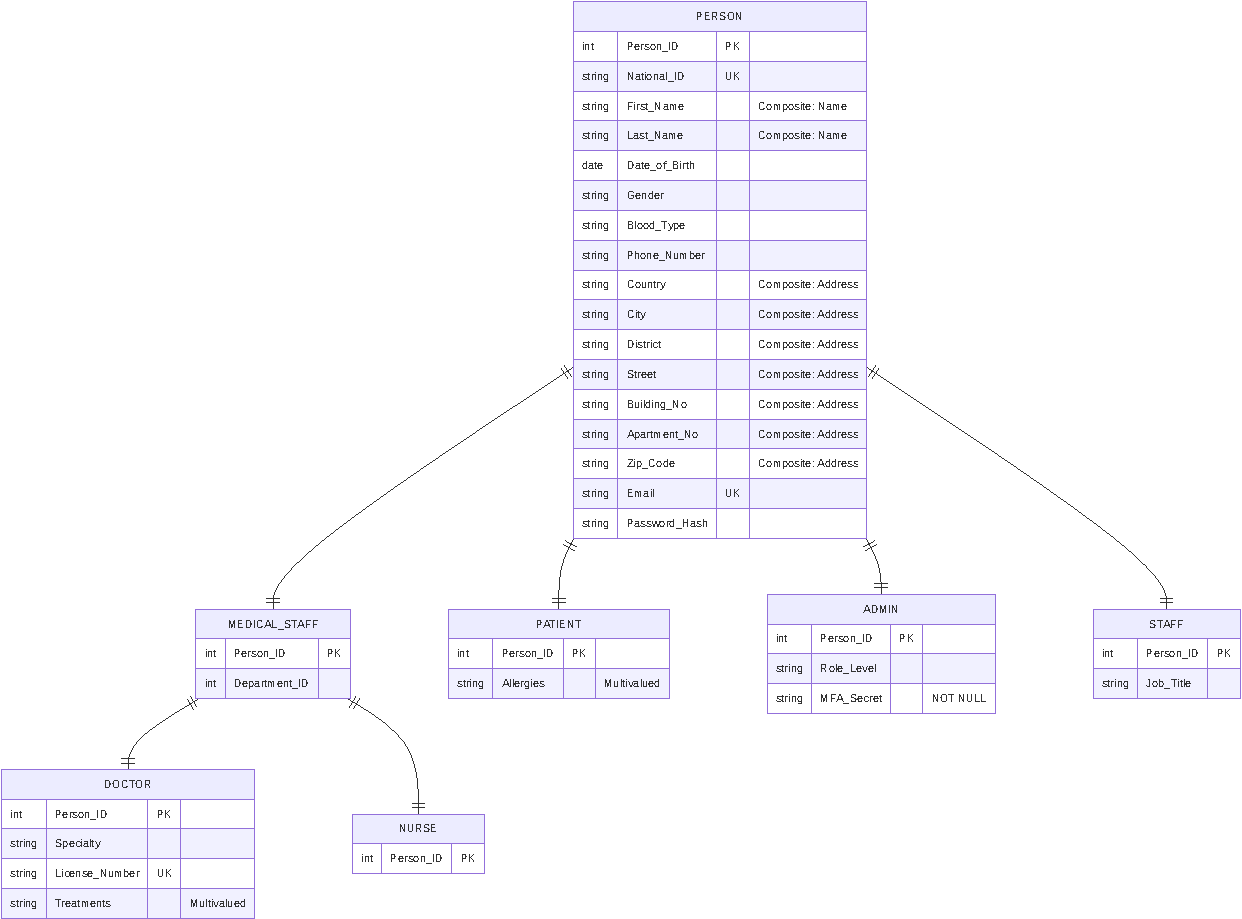
\includegraphics[width=1.2\textwidth, height=0.8\textheight]{Spec_Hierarchy.pdf}}
	\caption{Specialization/Generalization Hierarchy}
	\label{fig:spec_hier}
\end{figure}

\subsection{Conceptual Data Model}

\begin{figure}[H]
	\centering
	\makebox[\textwidth][c]{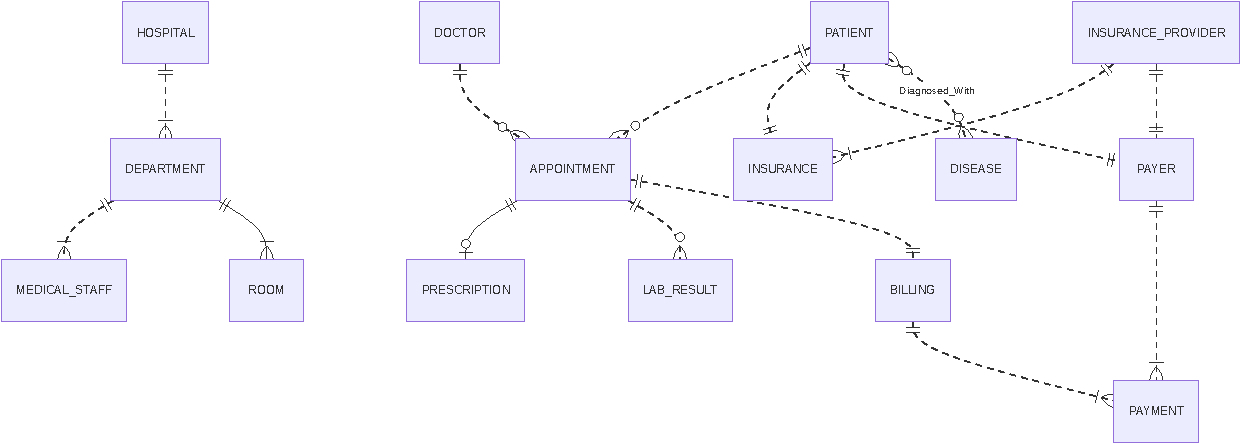
\includegraphics[width=1.2\textwidth, height=0.88\textheight]{Conceptual_Data_Model.pdf}}
	\caption{Conceptual Data Model}
	\label{fig:cd_model}
\end{figure}


\subsection{EER Diagram}

\begin{figure}[H]
	\centering
	\makebox[\textwidth][c]{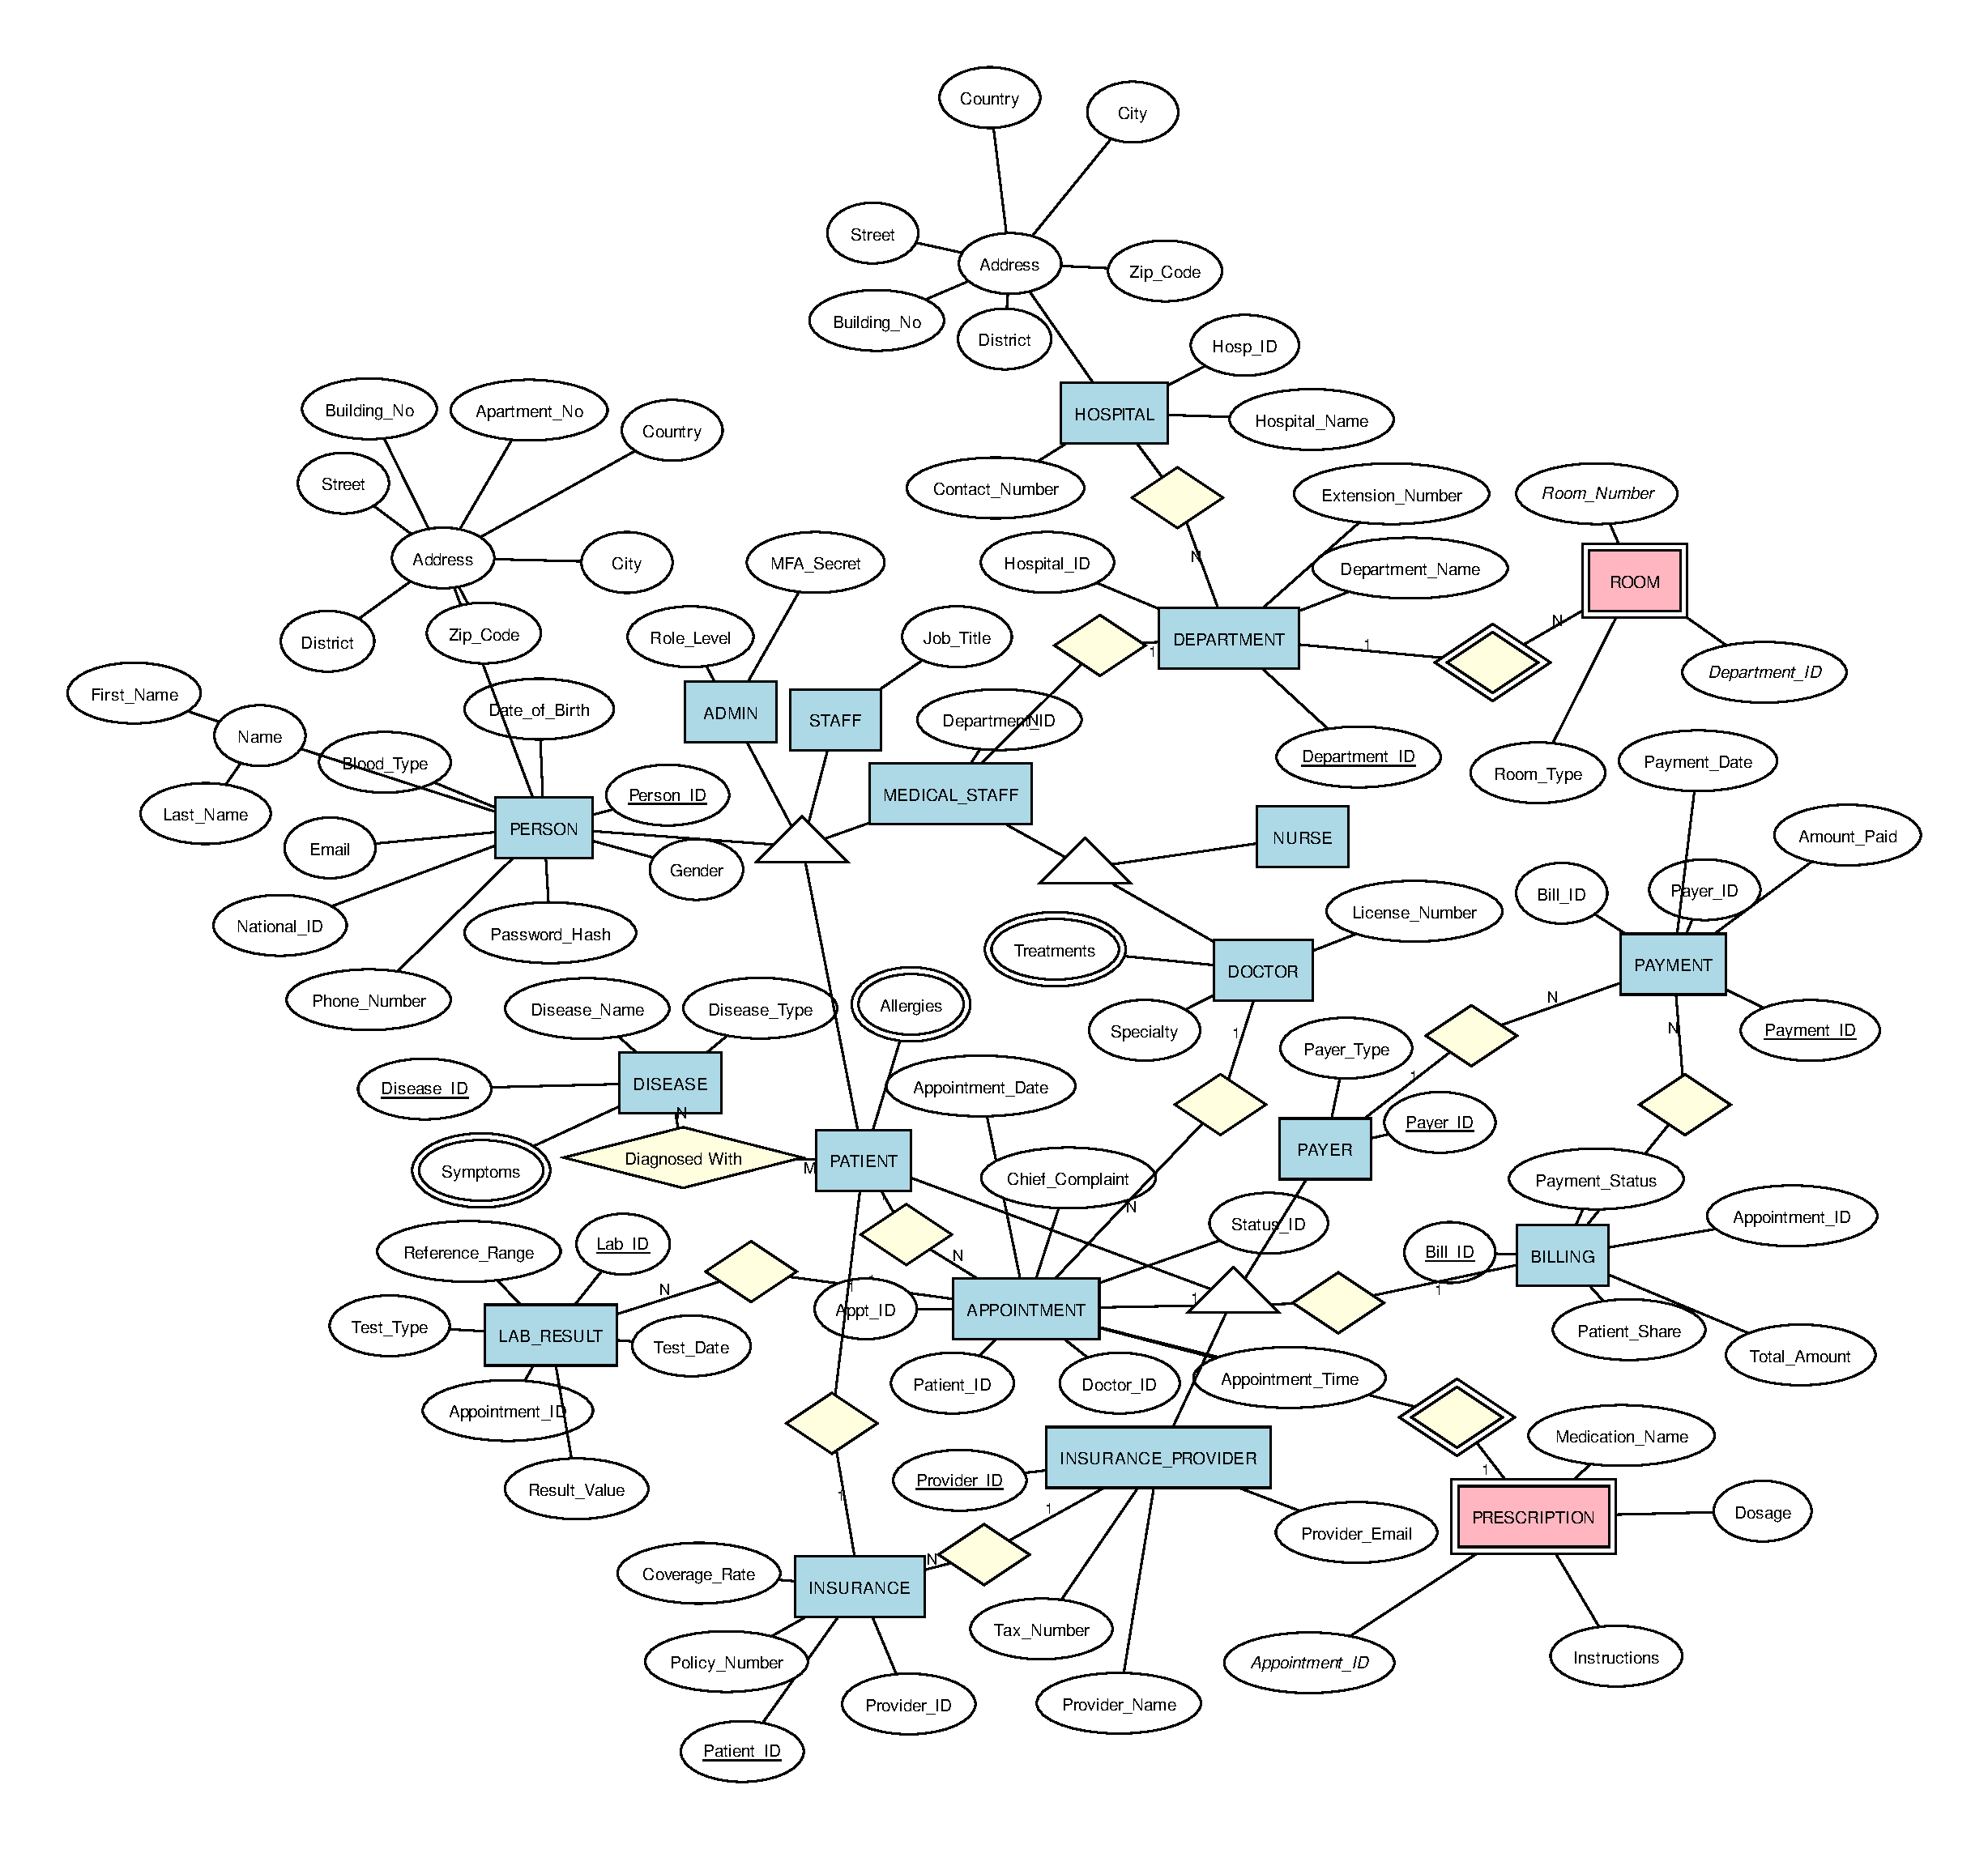
\includegraphics[width=1.2\textwidth, height=0.88\textheight]{EER_Diagram.pdf}}
	\caption{EER Diagram}
	\label{fig:eer_diagram}
\end{figure}


\section{Mapping to Relational Model}

In this phase, the conceptual Extended Entity-Relationship (EER) model is logically mapped into a relational database schema. The mapping strictly adheres to relational model constraints, specifically achieving First Normal Form (1NF) by eliminating multivalued attributes and composite attributes.
\subsection{Standard Entities and Hierarchical Mapping}
To maintain relational integrity and a clean architectural overview, all standard entities and hierarchical inheritance structures are mapped below by focusing strictly on their structural bones: Primary Keys (PK) and Foreign Keys (FK). All non-key descriptive attributes are omitted in this view to highlight the underlying relational connectivity.

\begin{itemize}[label=\textbf{--}]

	\item \textbf{PERSON}
	      \begin{itemize}[label=$\bullet$]
		      \item \texttt{Person\_ID} : \textit{Primary Key}
	      \end{itemize}

	\item \textbf{MEDICAL\_STAFF}
	      \begin{itemize}[label=$\bullet$]
		      \item \texttt{Person\_ID} : \textit{Primary Key, Foreign Key}
		      \item \texttt{Department\_ID} : \textit{Foreign Key}
	      \end{itemize}

	\item \textbf{PATIENT}
	      \begin{itemize}[label=$\bullet$]
		      \item \texttt{Person\_ID} : \textit{Primary Key, Foreign Key}
	      \end{itemize}

	\item \textbf{DOCTOR}
	      \begin{itemize}[label=$\bullet$]
		      \item \texttt{Person\_ID} : \textit{Primary Key, Foreign Key}
		      \item \texttt{License\_Number}\textsuperscript{UNIQUE}
	      \end{itemize}

	\item \textbf{NURSE}
	      \begin{itemize}[label=$\bullet$]
		      \item \texttt{Person\_ID} : \textit{Primary Key, Foreign Key}
	      \end{itemize}

	\item \textbf{ADMIN}
	      \begin{itemize}[label=$\bullet$]
		      \item \texttt{Person\_ID} : \textit{Primary Key, Foreign Key}
	      \end{itemize}

	\item \textbf{STAFF}
	      \begin{itemize}[label=$\bullet$]
		      \item \texttt{Person\_ID} : \textit{Primary Key, Foreign Key}
	      \end{itemize}

	\item \textbf{HOSPITAL}
	      \begin{itemize}[label=$\bullet$]
		      \item \texttt{Hospital\_ID} : \textit{Primary Key}
	      \end{itemize}

	\item \textbf{DEPARTMENT}
	      \begin{itemize}[label=$\bullet$]
		      \item \texttt{Department\_ID} : \textit{Primary Key}
		      \item \texttt{Hospital\_ID} : \textit{Foreign Key}
	      \end{itemize}

	\item \textbf{DISEASE}
	      \begin{itemize}[label=$\bullet$]
		      \item \texttt{Disease\_ID} : \textit{Primary Key}
	      \end{itemize}

	\item \textbf{LAB\_RESULT}
	      \begin{itemize}[label=$\bullet$]
		      \item \texttt{Lab\_ID} : \textit{Primary Key}
		      \item \texttt{Appointment\_ID} : \textit{Foreign Key}
	      \end{itemize}

	\item \textbf{INSURANCE\_PROVIDER}
	      \begin{itemize}[label=$\bullet$]
		      \item \texttt{Provider\_ID} : \textit{Primary Key}
	      \end{itemize}

	\item \textbf{INSURANCE}
	      \begin{itemize}[label=$\bullet$]
		      \item \texttt{Patient\_ID} : \textit{Primary Key, Foreign Key}
		      \item \texttt{Provider\_ID} : \textit{Foreign Key}
	      \end{itemize}

	\item \textbf{PAYER}
	      \begin{itemize}[label=$\bullet$]
		      \item \texttt{Payer\_ID} : \textit{Primary Key}
	      \end{itemize}

	\item \textbf{BILLING}
	      \begin{itemize}[label=$\bullet$]
		      \item \texttt{Bill\_ID} : \textit{Primary Key}
		      \item \texttt{Appointment\_ID} : \textit{Foreign Key}
	      \end{itemize}

	\item \textbf{PAYMENT}
	      \begin{itemize}[label=$\bullet$]
		      \item \texttt{Payment\_ID} : \textit{Primary Key}
		      \item \texttt{Bill\_ID} : \textit{Foreign Key}
		      \item \texttt{Payer\_ID} : \textit{Foreign Key}
	      \end{itemize}

\end{itemize}
\subsection{Handling Multivalued Attributes}
To comply with 1NF, multivalued attributes (\texttt{Allergies}, \texttt{Treatments}, \texttt{Symptoms}) are extracted from their parent entities and mapped into new, independent relations. The primary key of these new relations is a composite of the parent's primary key and the attribute value itself.

\begin{itemize}[label=\textbf{--}]

	\item \textbf{PATIENT\_ALLERGIES}
	      \begin{itemize}[label=$\bullet$]
		      \item \texttt{Person\_ID} : \textit{Primary Key, Foreign Key}
		      \item \texttt{Allergy\_Name} : \textit{Primary Key}
	      \end{itemize}

	\item \textbf{DOCTOR\_TREATMENTS}
	      \begin{itemize}[label=$\bullet$]
		      \item \texttt{Person\_ID} : \textit{Primary Key, Foreign Key}
		      \item \texttt{Treatment\_Name} : \textit{Primary Key}
	      \end{itemize}

	\item \textbf{DISEASE\_SYMPTOMS}
	      \begin{itemize}[label=$\bullet$]
		      \item \texttt{Disease\_ID} : \textit{Primary Key, Foreign Key}
		      \item \texttt{Symptom\_Name} : \textit{Primary Key}
	      \end{itemize}

\end{itemize}

\subsection{Mapping Weak Entities}
Weak entities cannot exist independently. They are mapped by absorbing the primary key of their owning entity as a foreign key, which then acts as part of their composite primary key (or sole primary key in 1:1 identifying relationships).

\begin{itemize}[label=\textbf{--}]

	\item \textbf{ROOM}
	      \begin{itemize}[label=$\bullet$]
		      \item \texttt{Department\_ID} : \textit{Primary Key, Foreign Key}
		      \item \texttt{Room\_Number} : \textit{Primary Key}
		      \item \texttt{Room\_Type}
	      \end{itemize}

	\item \textbf{PRESCRIPTION}
	      \begin{itemize}[label=$\bullet$]
		      \item \texttt{Appointment\_ID} : \textit{Primary Key, Foreign Key}
		      \item \texttt{Medication\_Name}
		      \item \texttt{Dosage}
		      \item \texttt{Instructions}
	      \end{itemize}

\end{itemize}

\subsection{Resolving Many-to-Many (M:N) Relationships}
M:N relationships are resolved by creating associative (junction) tables that contain foreign keys referencing the primary keys of the participating entities.

\begin{itemize}[label=\textbf{--}]

	\item \textbf{APPOINTMENT}
	      \begin{itemize}[label=$\bullet$]
		      \item \texttt{Appointment\_ID} : \textit{Primary Key}
		      \item \texttt{Patient\_ID} : \textit{Foreign Key}
		      \item \texttt{Doctor\_ID} : \textit{Foreign Key}
		      \item \texttt{Appointment\_Date}
		      \item \texttt{Appointment\_Time}
		      \item \texttt{Status\_ID}
		      \item \texttt{Chief\_Complaint}
	      \end{itemize}
	      \textit{(Resolves the implicit M:N relationship between Patient and Doctor.)}

	\item \textbf{DIAGNOSED\_WITH}
	      \begin{itemize}[label=$\bullet$]
		      \item \texttt{Patient\_ID} : \textit{Primary Key, Foreign Key}
		      \item \texttt{Disease\_ID} : \textit{Primary Key, Foreign Key}
		      \item \texttt{Diagnosis\_Date}
		      \item \texttt{Diagnosed\_Status}
	      \end{itemize}
	      \textit{(Resolves the M:N relationship between Patient and Disease.)}

\end{itemize}

\newpage
\begin{landscape}
	\thispagestyle{empty}
	\subsection{Relational Database Schema}
	\begin{center}
		\includegraphics[page=2, trim=0cm 2cm 0cm 2cm, clip, width=\linewidth]{DB_Schema.pdf}
		\captionof{figure}{Relational Database Schema}
		\label{fig:db_schema}
	\end{center}
\end{landscape}

\section{Functional Dependencies}
In this section, functional dependencies (FDs) are identified for three foundational tables that represent the biological, physical, and operational roots of the system: \textbf{PERSON}, \textbf{HOSPITAL}, and \textbf{APPOINTMENT}.

\subsubsection*{1. PERSON Table}
\texttt{PERSON} table is the hierarchical root of all individuals in the system. \texttt{Person\_ID} is the surrogate primary key and strictly determines all biological and contact attributes. Furthermore, since \texttt{National\_ID} (Citizen ID) and \texttt{Email} are enforced as globally unique constraints, they serve as \textit{Candidate Keys}. Therefore, they can also uniquely determine all other attributes in the relation independently.

\begin{itemize}[label=$\bullet$]
	\item $ \texttt{Person\_ID} \rightarrow \texttt{National\_ID}, \texttt{First\_Name}, \texttt{Last\_Name}, \texttt{Date\_of\_Birth}, \texttt{Gender}, \texttt{Blood\_Type}, \texttt{Email}, \dots $
	\item $ \texttt{National\_ID} \rightarrow \texttt{Person\_ID}, \texttt{First\_Name}, \texttt{Last\_Name}, \texttt{Email}, \dots $
	\item $ \texttt{Email} \rightarrow \texttt{Person\_ID}, \texttt{National\_ID}, \texttt{First\_Name}, \dots $
\end{itemize}

\subsubsection*{2. HOSPITAL Table}
\texttt{HOSPITAL} table defines the physical healthcare facilities. The primary key \texttt{Hospital\_ID} functionally determines the name, contact details, and the full composite address of the facility. A hospital's ID is completely sufficient to derive its exact physical location.

\begin{itemize}[label=$\bullet$]
	\item $ \texttt{Hospital\_ID} \rightarrow \texttt{Hospital\_Name}, \texttt{Contact\_Number}, \texttt{Country}, \texttt{City}, \texttt{District}, \texttt{Street}, \texttt{Building\_No}, \texttt{Zip\_Code} $
\end{itemize}

\subsubsection*{3. APPOINTMENT Table}
The \texttt{APPOINTMENT} table is the operational core connecting patients and doctors. While the primary key \texttt{Appointment\_ID} determines all operational details of a session, there is a strict operational business rule: \textit{A specific doctor cannot have two different appointments at the exact same date and time}. Thus, the composite of $(\texttt{Doctor\_ID}, \texttt{Appointment\_Date}, \texttt{Appointment\_Time})$ acts as a powerful candidate key that functionally determines the exact appointment, including who the patient is and what the complaint is.

\begin{itemize}[label=$\bullet$]
	\item $ \texttt{Appointment\_ID} \rightarrow \texttt{Patient\_ID}, \texttt{Doctor\_ID}, \texttt{Appointment\_Date}, \texttt{Appointment\_Time}, \texttt{Status\_ID}, \texttt{Chief\_Complaint} $
	\item $ \texttt{Doctor\_ID}, \texttt{Appointment\_Date}, \texttt{Appointment\_Time} \rightarrow \texttt{Appointment\_ID}, \texttt{Patient\_ID}, \texttt{Status\_ID}, \texttt{Chief\_Complaint} $
\end{itemize}

\section{Normalization}
Normalization is the formal mathematical process of analyzing relational schemas based on their functional dependencies (FDs) and primary keys to minimize data redundancy and eliminate insertion, deletion, and update anomalies.


\subsection{First Normal Form (1NF)}
A relation $R$ is in 1NF if all attributes contain only atomic values. This implies that each cell in the table must contain a single, indivisible value from the attribute's domain, effectively forbidding multi-valued attributes or nested relations.

The existing system satisfies 1NF as every attribute in all relations contains only atomic values.
\begin{itemize}[label=$\bullet$]
	\item \textbf{Atomicity:} Attributes such as \textit{Patient\_Name}, \textit{Doctor\_Specialty}, and \textit{Room\_Number} hold single values for each tuple.
	\item \textbf{Elimination of Multi-valued Attributes:} Multi-valued attributes like \textit{Allergies} or \textit{Symptoms} are not stored as arrays or comma-separated strings within the \texttt{PATIENT} or \texttt{APPOINTMENT} tables. Instead, they are decomposed into separate weak entities or associative tables (e.g., \texttt{PATIENT\_ALLERGY}), ensuring that $\forall t \in R, t[A]$ is atomic.
\end{itemize}

If we stored patient allergies directly within the \texttt{PATIENT} relation as a multi-valued attribute.

\begin{table}[h]
	\centering
	\begin{tabular}{llll}
		\toprule
		\textbf{Patient\_ID} & \textbf{Name} & \textbf{BirthDate} & \textbf{Allergies (Violation)}       \\
		\midrule
		P101                 & John Doe      & 1985-04-12         & \textcolor{red}{Penicillin, Peanuts} \\
		P102                 & Jane Smith    & 1992-08-25         & \textcolor{red}{Sulfur, Dust}        \\
		\bottomrule
	\end{tabular}
	\caption{Non-1NF Table: Multi-valued attributes cause search anomalies.}
\end{table}
To satisfy 1NF, the multi-valued attribute is decomposed into a separate weak entity, ensuring domain atomicity.

\begin{table}[h]
	\centering
	\begin{tabular}{ll}
		\toprule
		\textbf{Patient\_ID (FK)} & \textbf{Allergy\_Name} \\
		\midrule
		P101                      & Penicillin             \\
		P101                      & Peanuts                \\
		P102                      & Sulfur                 \\
		P102                      & Dust                   \\
		\bottomrule
	\end{tabular}
	\caption{1NF Compliant: Decomposed \texttt{PATIENT\_ALLERGY} relation.}
\end{table}


\subsection{Second Normal Form (2NF)}
A relation $R$ is in 2NF if it is in 1NF and every non-prime attribute is fully functionally dependent on the entire primary key. This prevents partial functional dependencies, where an attribute depends only on a subset of a composite primary key rather than the key in its entirety.

A relation violates 2NF only if it has a composite primary key and a partial dependency exists.
\begin{itemize}[label=$\bullet$]
	\item \textbf{Single-Attribute Keys:} Most critical tables (e.g., \texttt{PATIENT}, \texttt{DOCTOR}, \texttt{DEPARTMENT}) utilize a single-attribute primary key (Surrogate Keys like \textit{Patient\_ID}). Since a proper subset of a single-attribute key is an empty set, partial functional dependency is mathematically impossible.
	\item \textbf{Composite Keys:} In relations with composite keys, such as \texttt{APPOINTMENT (Doctor\_ID, Start\_Time)}, all non-prime attributes like \textit{Diagnosis} or \textit{Status} are fully functionally dependent on the \textbf{entire} key. Knowledge of only \textit{Doctor\_ID} is insufficient to determine a specific \textit{Diagnosis} without the temporal context of \textit{Start\_Time}.
\end{itemize}

In our schema, we utilize a composite primary key to uniquely identify rooms, combining the Department and the Room itself: \textit{(Department\_ID, Room\_Number)}. If we had incorrectly included the department's name within this room-specific relation, a 2NF violation would occur.

\begin{table}[h]
	\centering
	\begin{tabular}{llll}
		\toprule
		\textbf{Department\_ID} & \textbf{Room\_Number} & \textbf{Department\_Name (Violation)} \\
		\midrule
		DEP-1                   & 101                   & \textcolor{red}{Cardiology}           \\
		DEP-1                   & 102                   & \textcolor{red}{Cardiology}           \\
		DEP-2                   & 101                   & \textcolor{red}{Neurology}            \\
		\bottomrule
	\end{tabular}
	\caption{Non-2NF Table: \textit{Department\_Name} is partially dependent only on \textit{Department\_ID}.}
\end{table}
To strictly adhere to 2NF, our actual design eliminates this partial dependency. The \textit{Department\_Name} is exclusively stored in the \texttt{DEPARTMENT} table. In our actual \texttt{ROOM} table, attributes such as \textit{Capacity} are fully functionally dependent on the \textbf{entire} composite key \textit{(Department\_ID, Room\_Number)}, preventing massive data redundancy.

\begin{table}[h]
	\centering
	\begin{tabular}{lll}
		\toprule
		\textbf{Department\_ID (PK/FK)} & \textbf{Room\_Number (PK)} \\
		\midrule
		DEP-1                           & 101                        \\
		DEP-1                           & 102                        \\
		DEP-2                           & 101                        \\
		\bottomrule
	\end{tabular}
	\caption{2NF Compliant: The actual \texttt{ROOM} relation without partial dependencies.}
\end{table}

\subsection{Third Normal Form (3NF)}
A relation schema $R$ is in third normal form with respect to a set $F$ of functional dependencies if, for all functional dependencies in $F^+$ of the form $\alpha \rightarrow \beta$, where $\alpha \subseteq R$ and $\beta \subseteq R$, at least one of the following holds:

\begin{itemize}[label=\textbf{--}]
	\item $\alpha \rightarrow \beta$ is a trivial functional dependency.
	\item $\alpha$ is a superkey for $R$.
	\item Each attribute $A$ in $\beta - \alpha$ is contained in a candidate key for $R$.
\end{itemize}

The schema eliminates transitive dependencies by ensuring that non-prime attributes are determined only by the primary key.
\begin{itemize}[label=$\bullet$]
	\item \textbf{Example:} In the \texttt{DOCTOR} relation, we store \textit{Department\_ID} but not \textit{Department\_Name} or \textit{Department\_Location}. If we had included \textit{Department\_Name}, a transitive dependency would exist: $Doctor\_ID \rightarrow Department\_ID \rightarrow Department\_Name$.
	\item By isolating Department details into a separate \texttt{DEPARTMENT} table, we ensure that for every $X \rightarrow A$, $X$ is a superkey, satisfying the 3NF requirements across the entire relational forest.
\end{itemize}

If the \texttt{DOCTOR} table stored both the Department ID and the physical location of that department.

\begin{table}[h]
	\centering
	\begin{tabular}{llll}
		\toprule
		\textbf{Doctor\_ID} & \textbf{Name} & \textbf{Department\_ID} & \textbf{Location (Violation)}         \\
		\midrule
		D501                & Dr. Adams     & DEP-1                   & \textcolor{red}{Building A - Floor 3} \\
		D503                & Dr. Clark     & DEP-1                   & \textcolor{red}{Building A - Floor 3} \\
		\bottomrule
	\end{tabular}
	\caption{Non-3NF Table: Transitive dependency (\textit{Doctor\_ID} $\rightarrow$ \textit{Department\_ID} $\rightarrow$ \textit{Location}).}
\end{table}
To eliminate the transitive chain and prevent update anomalies (e.g., if a department moves to a new floor), \textit{Location} is completely isolated into the \texttt{DEPARTMENT} table.

\begin{table}[h]
	\centering
	\begin{tabular}{lll}
		\toprule
		\textbf{Department\_ID (PK)} & \textbf{Department\_Name} & \textbf{Location}    \\
		\midrule
		DEP-1                        & Cardiology                & Building A - Floor 3 \\
		DEP-2                        & Neurology                 & Building B - Floor 1 \\
		\bottomrule
	\end{tabular}
	\caption{3NF Compliant: Decomposed \texttt{DEPARTMENT} relation.}
\end{table}

\subsection{Boyce-Codd Normal Form (BCNF)}
A relation schema $R$ is in BCNF with respect to a set $F$ of functional dependencies if, for all functional dependencies in $F^+$ of the form $\alpha \rightarrow \beta$, where $\alpha \subseteq R$ and $\beta \subseteq R$, at least one of the following holds:

\begin{itemize}[label=\textbf{--}]
	\item $\alpha \rightarrow \beta$ is a trivial functional dependency (i.e., $\beta \subseteq \alpha$).
	\item $\alpha$ is a superkey for schema $R$.
\end{itemize}

The schema reaches BCNF, the strictest of the functional dependency-based forms, as the only determinants in our functional dependency set $F$ are superkeys.
\begin{itemize}[label=$\bullet$]
	\item \textbf{Proof by Determinant Analysis:} Reviewing the FDs from Section 5:
	      \begin{itemize}
		      \item $Patient\_ID \rightarrow \{Name, BirthDate, Gender\}$: Determinant is a Primary Key/Superkey
		      \item $Doctor\_ID \rightarrow \{Name, Specialty, Department\_ID\}$ Determinant is a Primary Key/Superkey
		      \item $Room\_ID \rightarrow \{Room\_Number, Capacity\}$ Determinant is a Primary Key/Superkey
	      \end{itemize}
	\item Since there are no non-trivial functional dependencies $\alpha \rightarrow \beta$ where $\alpha$ is not a superkey, the system is inherently in BCNF. No prime attribute is functionally determined by a non-superkey.
\end{itemize}

For more information, see \href{https://github.com/mosquitozm100/JHU-EN.601.615-Databases/blob/master/Database%20System%20Concepts%2C%20Seventh%20Edition.pdf}{Database System Concepts by Silberschatz, Korth and Sudarshan, Chapter 7.3: Normal Forms}


\section{SQL Implementation}
\subsection{Data Definition Language (DDL) and Table Constraints}

\begin{lstlisting}[language=SQL, caption=Creating Database, basicstyle=\ttfamily\footnotesize, breaklines=true]
CREATE DATABASE smarthealth-db:
\end{lstlisting}

\vspace{0.3cm}
\begin{lstlisting}[language=SQL, caption=Core Schema Creation and Constraint Definitions, basicstyle=\ttfamily\footnotesize, breaklines=true]

-- SQL dump generated using DBML (dbml.dbdiagram.io)
-- Database: PostgreSQL

CREATE TABLE "Hospital" (
  "Hospital_ID" int PRIMARY KEY,
  "Hospital_Name" varchar,
  "Address_Country" varchar,
  "Address_City" varchar,
  "Address_District" varchar,
  "Address_Street" varchar,
  "Address_Building_No" varchar,
  "Address_Zip_Code" varchar,
  "Contact_Number" varchar
);

CREATE TABLE "Disease" (
  "Disease_ID" int PRIMARY KEY,
  "Disease_Name" varchar,
  "Disease_Type" varchar
);

CREATE TABLE "Disease_Symptom" (
  "Disease_ID" int REFERENCES "Disease" ("Disease_ID"),
  "Symptom_Name" varchar,
  PRIMARY KEY ("Disease_ID", "Symptom_Name")
);

CREATE TABLE "Insurance_Provider" (
  "Provider_ID" int PRIMARY KEY,
  "Provider_Name" varchar,
  "Tax_Number" varchar,
  "Provider_Email" varchar
);

CREATE TABLE "Person" (
  "Person_ID" int PRIMARY KEY,
  "National_ID" varchar UNIQUE,
  "Name_First_Name" varchar,
  "Name_Last_Name" varchar,
  "Date_of_Birth" date,
  "Gender" varchar,
  "Blood_Type" varchar,
  "Phone_Number" varchar,
  "Address_Country" varchar,
  "Address_City" varchar,
  "Address_District" varchar,
  "Address_Street" varchar,
  "Address_Building_No" varchar,
  "Address_Apartment_No" varchar,
  "Address_Zip_Code" varchar,
  "Email" varchar UNIQUE,
  "Password_Hash" varchar
);

CREATE TABLE "Department" (
  "Department_ID" int PRIMARY KEY,
  "Hospital_ID" int REFERENCES "Hospital" ("Hospital_ID"),
  "Department_Name" varchar,
  "Extension_Number" varchar
);

CREATE TABLE "Patient" (
  "Person_ID" int PRIMARY KEY REFERENCES "Person" ("Person_ID") 
);

CREATE TABLE "Patient_Allergy" (
  "Patient_ID" int REFERENCES "Patient" ("Person_ID"),
  "Allergy_Name" varchar,
  PRIMARY KEY ("Patient_ID", "Allergy_Name")
);

CREATE TABLE "Admin" (
  "Person_ID" int PRIMARY KEY REFERENCES "Person" ("Person_ID"),
  "Role_Level" varchar,
  "MFA_Secret" varchar NOT NULL
);

CREATE TABLE "Staff" (
  "Person_ID" int PRIMARY KEY REFERENCES "Person" ("Person_ID"),
  "Job_Title" varchar
);

CREATE TABLE "Medical_Staff" (
  "Person_ID" int PRIMARY KEY REFERENCES "Person" ("Person_ID"),
  "Department_ID" int REFERENCES "Department" ("Department_ID")
);

CREATE TABLE "Room" (
  "Department_ID" int REFERENCES "Department" ("Department_ID"),
  "Room_Number" varchar,
  "Room_Type" varchar,
  PRIMARY KEY ("Department_ID", "Room_Number")
);

CREATE TABLE "Doctor" (
  "Person_ID" int PRIMARY KEY REFERENCES "Medical_Staff" ("Person_ID"),
  "Specialty" varchar,
  "License_Number" varchar UNIQUE
);

CREATE TABLE "Doctor_Treatment" (
  "Doctor_ID" int REFERENCES "Doctor" ("Person_ID"),
  "Treatment_Name" varchar,
  PRIMARY KEY ("Doctor_ID", "Treatment_Name")
);

CREATE TABLE "Nurse" (
  "Person_ID" int PRIMARY KEY REFERENCES "Medical_Staff" ("Person_ID") 
);

CREATE TABLE "Payer" (
  "Payer_ID" int PRIMARY KEY,
  "Payer_Type" varchar CHECK ("Payer_Type" IN ('Patient', 'Insurance')),
  "Patient_ID" int REFERENCES "Patient" ("Person_ID"),
  "Provider_ID" int REFERENCES "Insurance_Provider" ("Provider_ID"),
  CONSTRAINT check_exclusive_payer CHECK (
    ("Payer_Type" = 'Patient' AND "Patient_ID" IS NOT NULL AND "Provider_ID" IS NULL) OR
    ("Payer_Type" = 'Insurance' AND "Provider_ID" IS NOT NULL AND "Patient_ID" IS NULL)
  )
);

CREATE TABLE "Insurance" (
  "Patient_ID" int REFERENCES "Patient" ("Person_ID"),
  "Provider_ID" int REFERENCES "Insurance_Provider" ("Provider_ID"),
  "Policy_Number" varchar,
  "Coverage_Rate" decimal CHECK ("Coverage_Rate" >= 0 AND "Coverage_Rate" <= 100),
  PRIMARY KEY ("Patient_ID", "Provider_ID")
);

CREATE TABLE "Patient_Disease" (
  "Patient_Person_ID" int REFERENCES "Patient" ("Person_ID"),
  "Disease_Disease_ID" int REFERENCES "Disease" ("Disease_ID"),
  PRIMARY KEY ("Patient_Person_ID", "Disease_Disease_ID")
);

CREATE TABLE "Appointment" (
  "Appointment_ID" int PRIMARY KEY,
  "Patient_ID" int REFERENCES "Patient" ("Person_ID"),
  "Doctor_ID" int REFERENCES "Doctor" ("Person_ID"),
  "Appointment_Date" date,
  "Appointment_Time" time,
  "Status_ID" int CHECK ("Status_ID" IN (0, 1, 2)),
  "Chief_Complaint" varchar
);

CREATE TABLE "Prescription" (
  "Appointment_ID" int PRIMARY KEY REFERENCES "Appointment" ("Appointment_ID"),
  "Medication_Name" varchar,
  "Dosage" varchar,
  "Instructions" varchar
);

CREATE TABLE "Lab_Result" (
  "Lab_ID" int PRIMARY KEY,
  "Appointment_ID" int REFERENCES "Appointment" ("Appointment_ID"),
  "Test_Type" varchar,
  "Result_Value" varchar,
  "Reference_Range" varchar,
  "Test_Date" date
);

CREATE TABLE "Billing" (
  "Bill_ID" int PRIMARY KEY,
  "Appointment_ID" int REFERENCES "Appointment" ("Appointment_ID"),
  "Total_Amount" decimal CHECK ("Total_Amount" >= 0),
  "Patient_Share" decimal CHECK ("Patient_Share" >= 0),
  "Payment_Status" int,
  CONSTRAINT check_share_limit CHECK ("Patient_Share" <= "Total_Amount")
);

CREATE TABLE "Payment" (
  "Payment_ID" int PRIMARY KEY,
  "Bill_ID" int REFERENCES "Billing" ("Bill_ID"),
  "Payer_ID" int REFERENCES "Payer" ("Payer_ID"),
  "Amount_Paid" decimal CHECK ("Amount_Paid" >= 0),
  "Payment_Date" timestamp
);

\end{lstlisting}

\subsection{Data Manipulation Language (DML) and Sample Data Entry}

To test the structural correctness of the designed relational database schema, data integrity constraints, and relational flow between tables, a sample dataset was injected into the system. The order in which the data was inserted was designed considering the foreign key dependency chain and topological hierarchy in the database. The `\texttt{INSERT}` commands prepared for system testing are presented below:
\begin{lstlisting}[language=SQL, caption=DML Script, basicstyle=\ttfamily\footnotesize, breaklines=true]


INSERT INTO "Hospital" (
  "Hospital_ID", 
  "Hospital_Name", 
  "Address_Country", 
  "Address_City", 
  "Address_District", 
  "Address_Street", 
  "Address_Building_No", 
  "Address_Zip_Code", 
  "Contact_Number"
) VALUES 
(1, 'Cerrahpasa Faculty of Medicine Hospital', 'Turkey', 'Istanbul', 'Fatih', 'Kocamustafapasa Ave.', '53', '34098', '+902124143000'),
(2, 'Acibadem Maslak Hospital', 'Turkey', 'Istanbul', 'Sariyer', 'Buyukdere Ave.', '40', '34457', '+902123044444'),
(3, 'Koc University Hospital', 'Turkey', 'Istanbul', 'Zeytinburnu', 'Davutpasa Ave.', '4', '34010', '+908502508250'),
(4, 'Hacettepe University Hospital', 'Turkey', 'Ankara', 'Altindag', 'Sihhiye', '1', '06230', '+903123055000'),
(5, 'Ege University Faculty of Medicine Hospital', 'Turkey', 'Izmir', 'Bornova', 'Ege University Campus', '1', '35100', '+902323901199'),
(6, 'St Thomas Hospital', 'United Kingdom', 'London', 'Lambeth', 'Westminster Bridge Rd', '1', 'SE1 7EH', '+442071887188'),
(7, 'The Mount Sinai Hospital', 'United States', 'New York', 'Manhattan', 'Gustave L. Levy Pl', '1', '10029', '+12122416500'),
(8, 'Charite - Universitatsmedizin', 'Germany', 'Berlin', 'Mitte', 'Chariteplatz', '1', '10117', '+493045050');

INSERT INTO "Disease" (
  "Disease_ID", 
  "Disease_Name", 
  "Disease_Type"
) VALUES 
(1, 'Type 2 Diabetes', 'Chronic'),
(2, 'Hypertension', 'Cardiovascular'),
(3, 'COVID-19', 'Infectious'),
(4, 'Asthma', 'Chronic'),
(5, 'Rheumatoid Arthritis', 'Autoimmune'),
(6, 'Tuberculosis', 'Infectious'),
(7, 'Alzheimer', 'Neurological'),
(8, 'Influenza (Flu)', 'Infectious'),
(9, 'Leukemia', 'Oncological'),
(10, 'Migraine', 'Neurological');

INSERT INTO "Insurance_Provider" (
  "Provider_ID", 
  "Provider_Name", 
  "Tax_Number", 
  "Provider_Email"
) VALUES 
(1, 'Social Security Institution (SGK)', '7720394320', 'contact@sgk.gov.tr'),
(2, 'Allianz Insurance', '0550009620', 'info@allianz.com.tr'),
(3, 'Anadolu Insurance', '0680061327', 'bilgi@anadolusigorta.com.tr'),
(4, 'Bupa Acibadem Insurance', '0070081580', 'info@bupaacibadem.com.tr'),
(5, 'National Health Service (NHS)', 'GB123456789', 'england.contactus@nhs.net'),
(6, 'Medicare', 'US987654321', 'medicare.support@cms.hhs.gov'),
(7, 'Cigna Global', 'GB987654321', 'cignaglobal_customer.care@cigna.com'),
(8, 'Techniker Krankenkasse (TK)', 'DE123456789', 'service@tk.de');

-- Remaining data entries can be found in the sql/data_sample.sql file

\end{lstlisting}

\subsection{ALTER Operations}

To test the flexibility and evolutionary capacity of the database schema in the live environment, various `\texttt{ALTER}` operations were performed. These operations allowed the addition of new business rules and fields to the schema while maintaining the integrity of existing data in the system.
\begin{lstlisting}[language=SQL, caption=Database Schema Modification Operations, basicstyle=\ttfamily\footnotesize, breaklines=true]

ALTER TABLE "Person" ADD COLUMN "Emergency_Contact" varchar;


ALTER TABLE "Appointment" ALTER COLUMN "Status_ID" SET DEFAULT 0;


ALTER TABLE "Billing" ADD CONSTRAINT check_min_bill CHECK ("Total_Amount" >= 50) NOT VALID;
\end{lstlisting}


\section{Advanced SQL Queries}
\setcounter{figure}{0}
\renewcommand{\thefigure}{\arabic{figure}}

\begin{figure}[H]
	\centering
	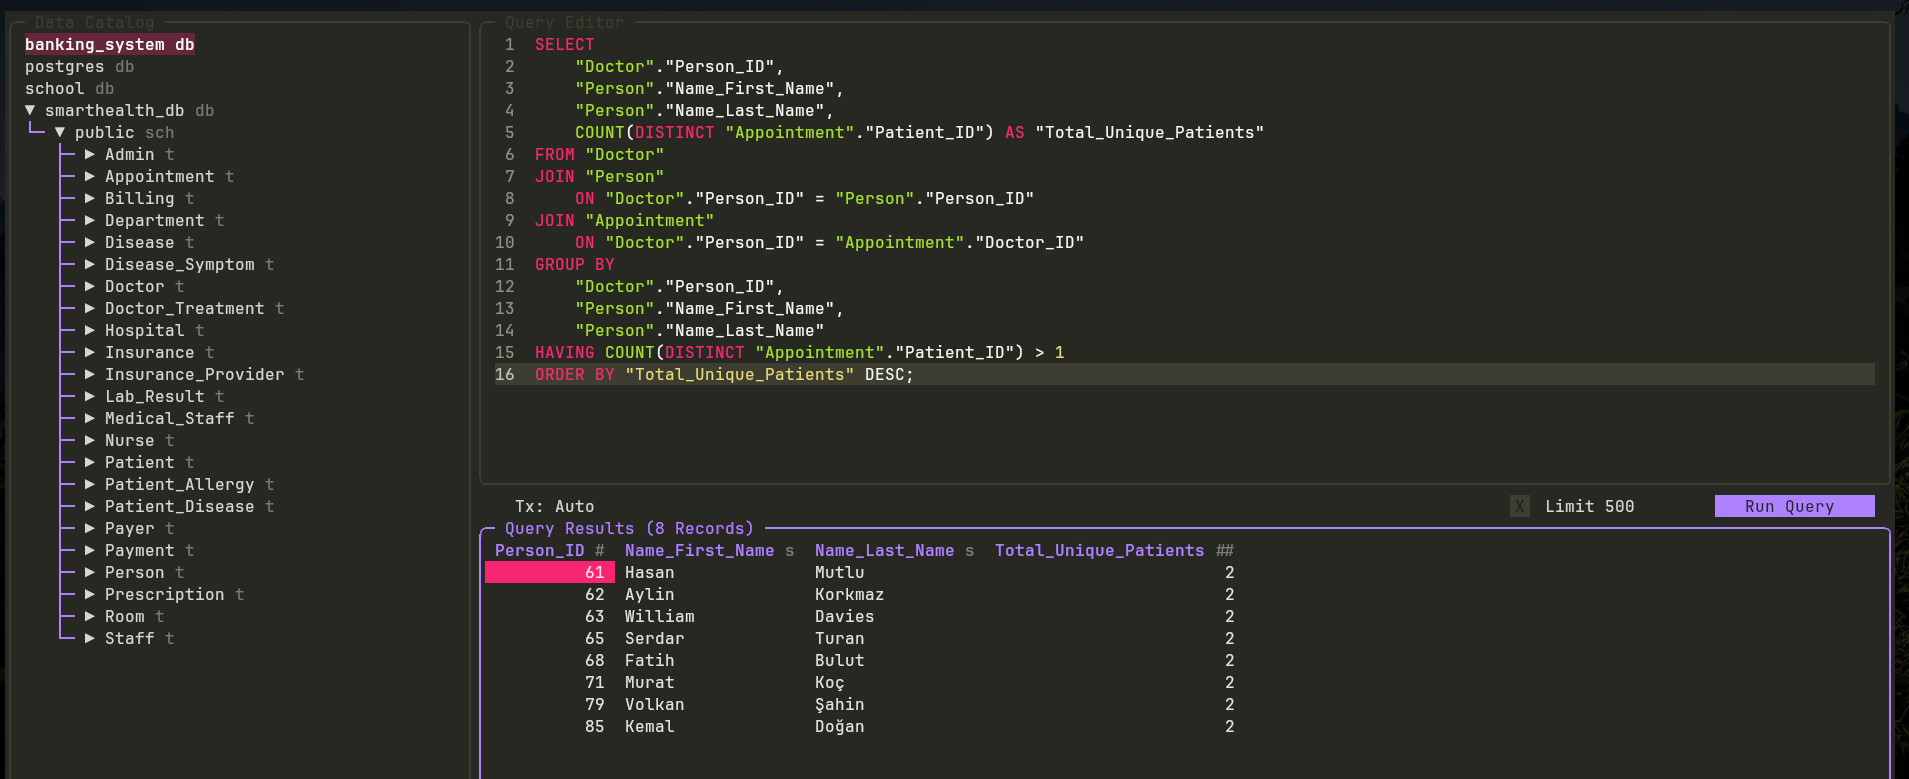
\includegraphics[width=0.8\textwidth]{query_01.png}
	\caption{Doctors who see more than one patient}
\end{figure}

\begin{figure}[H]
	\centering
	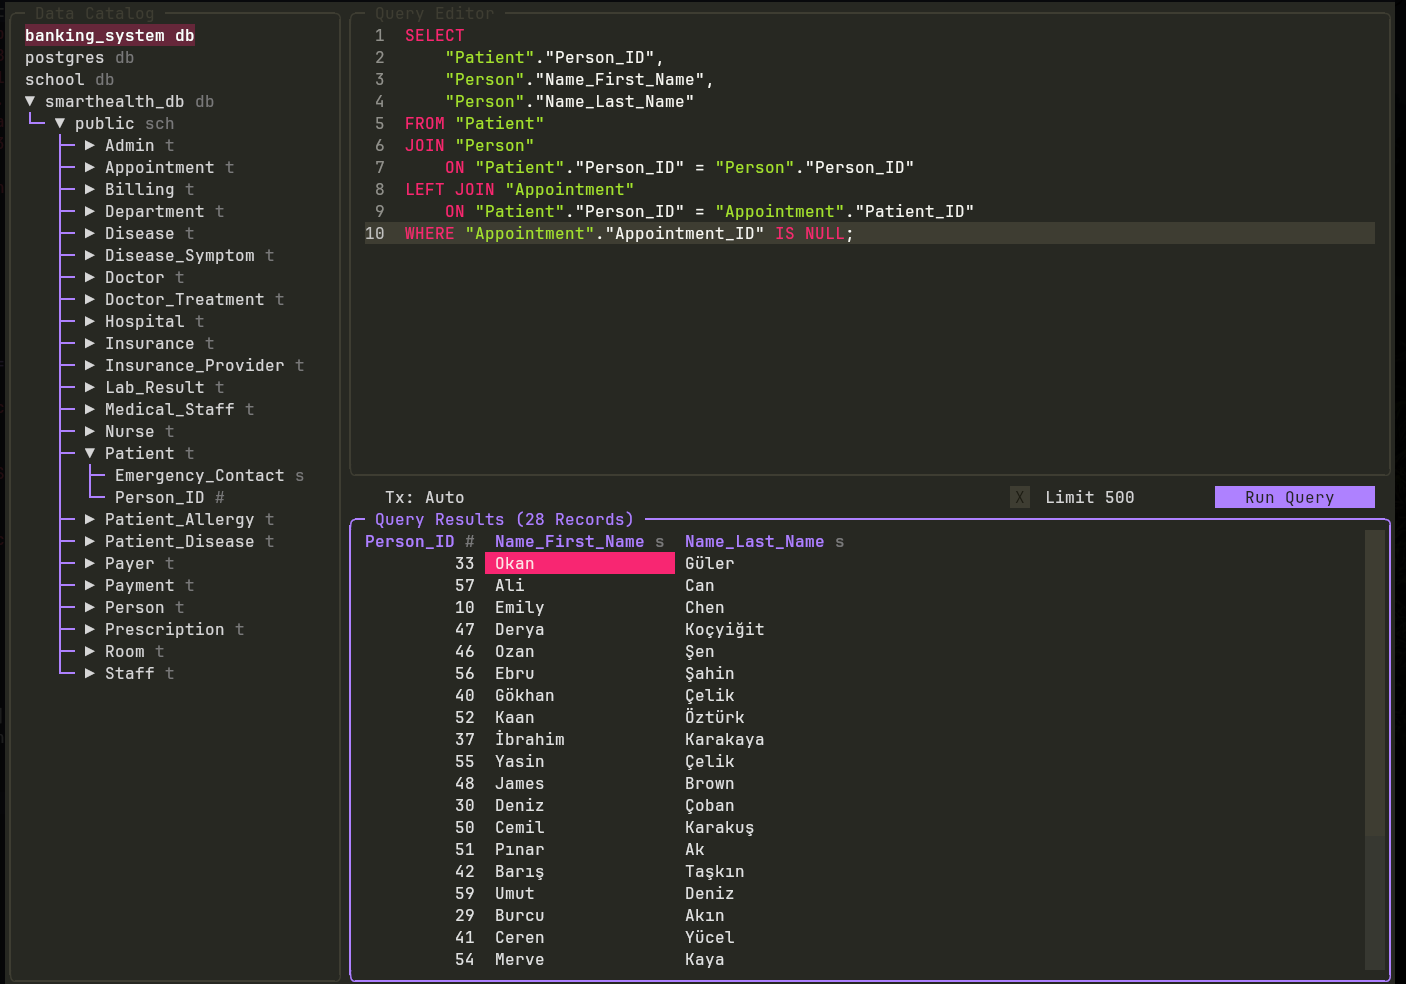
\includegraphics[width=0.8\textwidth]{query_02.png}
	\caption{Patients with no appointments}
\end{figure}

\begin{figure}[H]
	\centering
	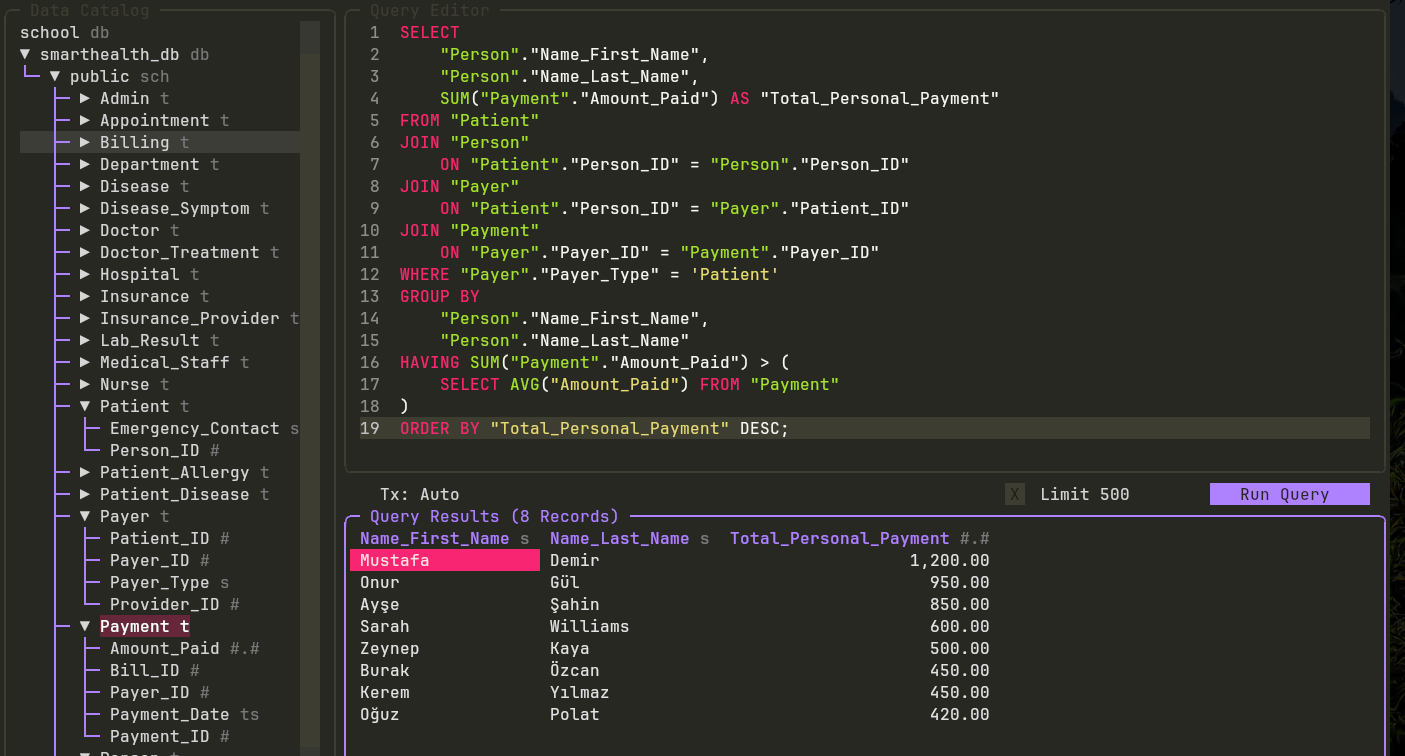
\includegraphics[width=0.8\textwidth]{query_03.png}
	\caption{Patients who pay above average}
\end{figure}

\begin{figure}[H]
	\centering
	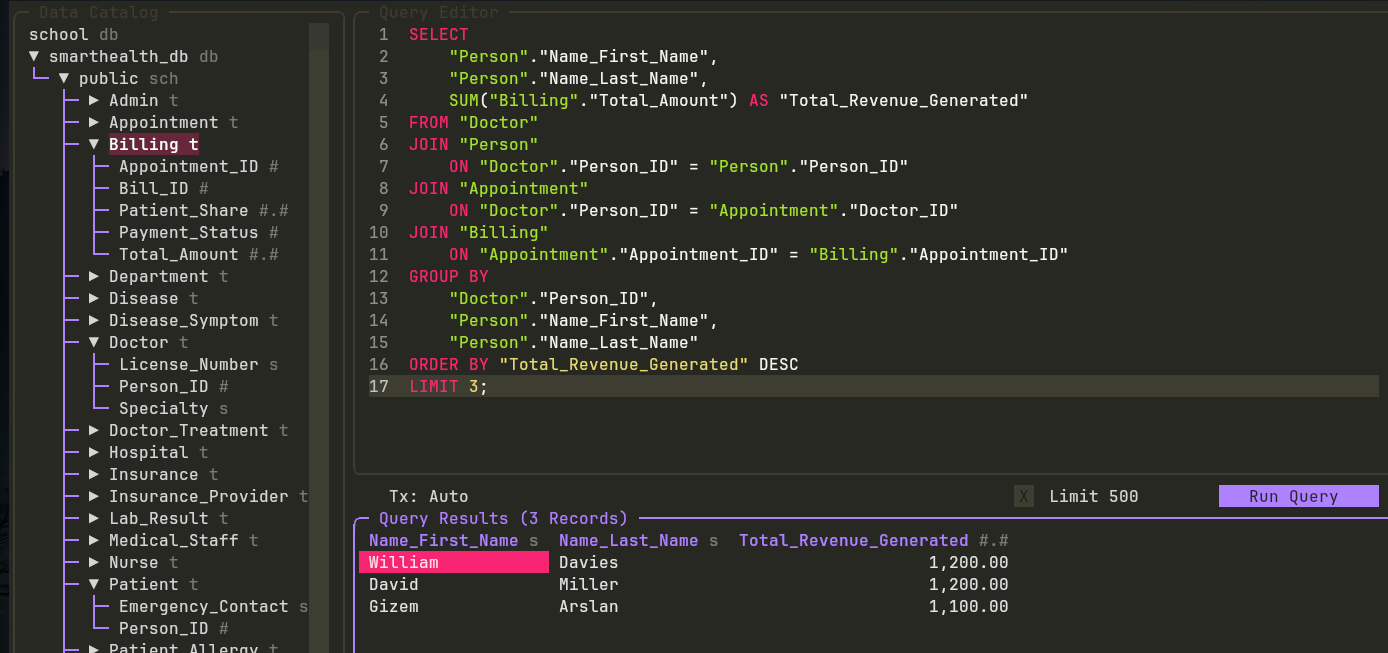
\includegraphics[width=0.8\textwidth]{query_04.png}
	\caption{3 doctors who generate the most revenue for the hospital}
\end{figure}

\begin{figure}[H]
	\centering
	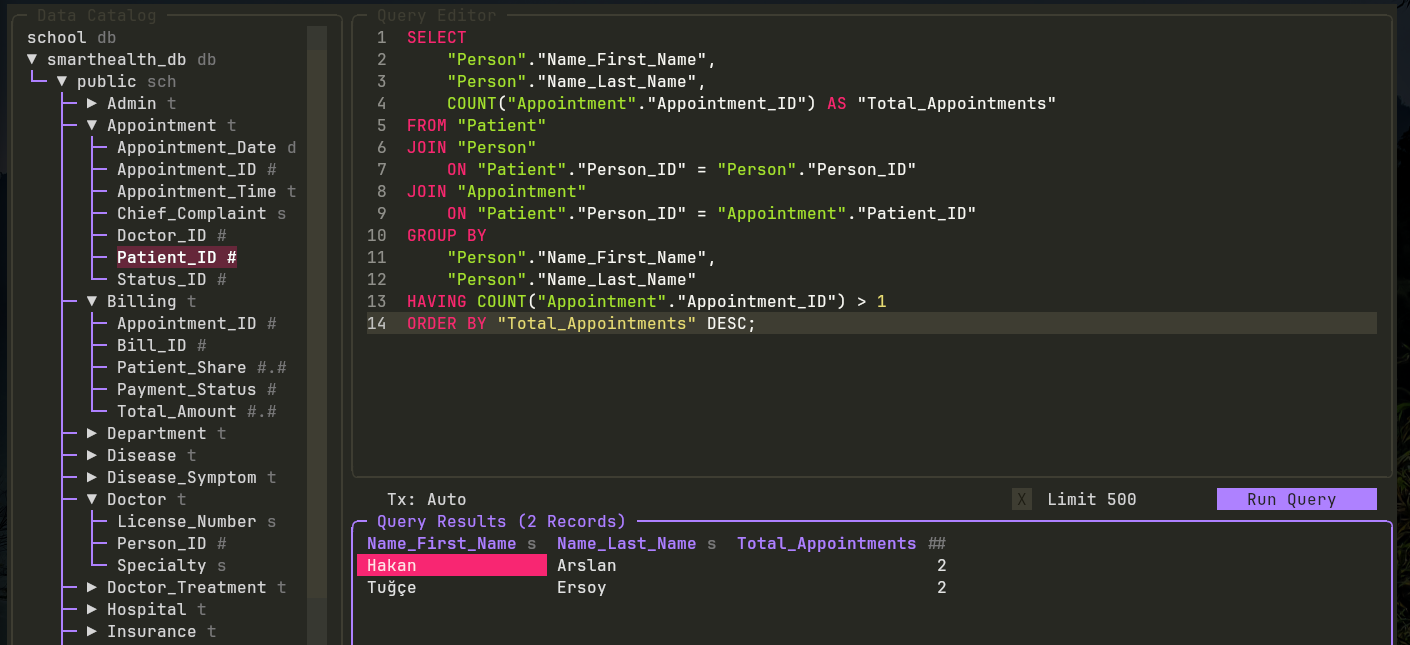
\includegraphics[width=0.8\textwidth]{query_05.png}
	\caption{Patients with multiple appointments}
\end{figure}

\begin{figure}[H]
	\centering
	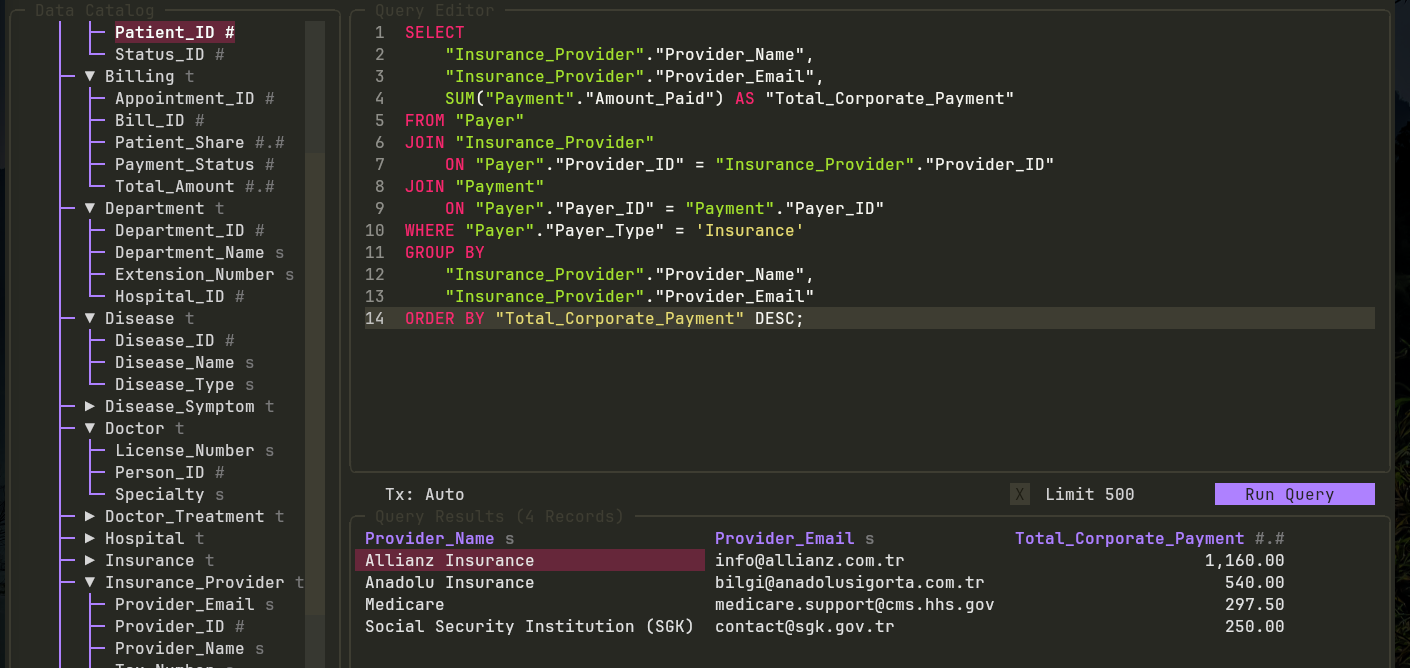
\includegraphics[width=0.8\textwidth]{query_06.png}
	\caption{List of insurance providers that make payments}
\end{figure}

\begin{figure}[H]
	\centering
	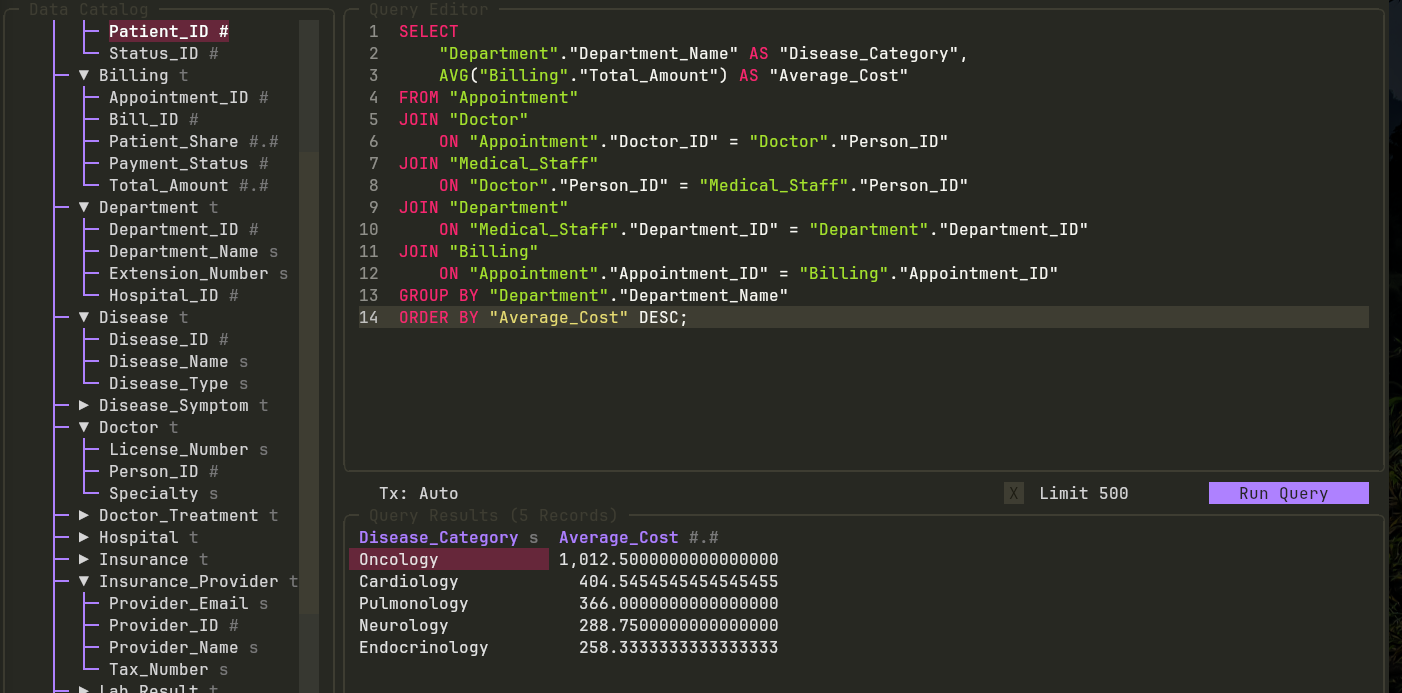
\includegraphics[width=0.8\textwidth]{query_07.png}
	\caption{Average cost per appointment for each department}
\end{figure}

\begin{figure}[H]
	\centering
	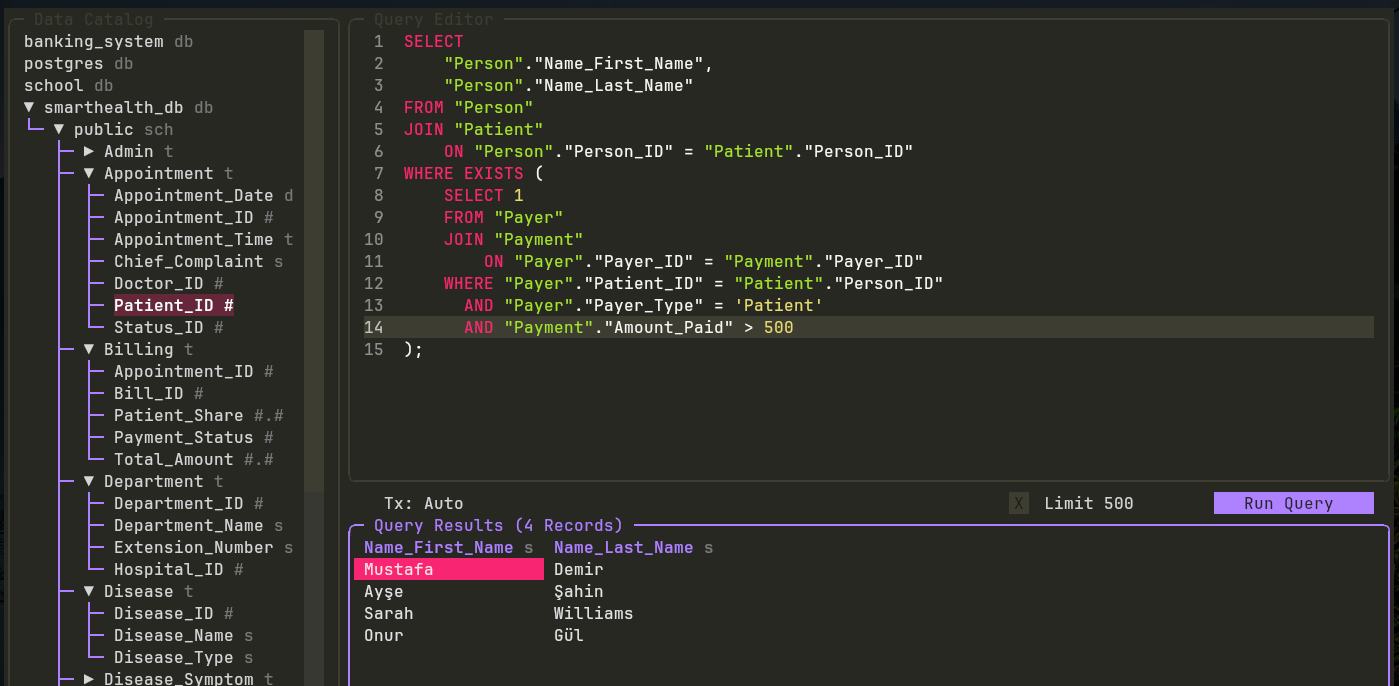
\includegraphics[width=0.8\textwidth]{query_08.png}
	\caption{Patients who made a single payment of more than 500}
\end{figure}

\begin{figure}[H]
	\centering
	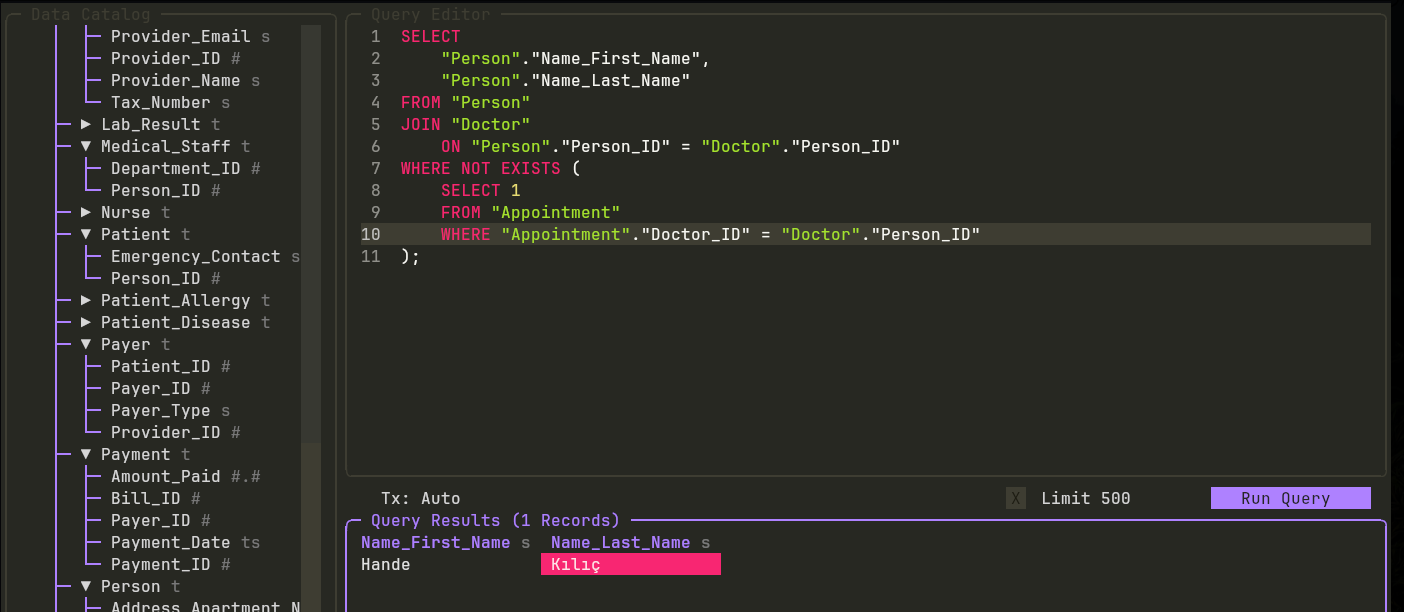
\includegraphics[width=0.8\textwidth]{query_09.png}
	\caption{That one doctor who have no appointments}
\end{figure}

\begin{figure}[H]
	\centering
	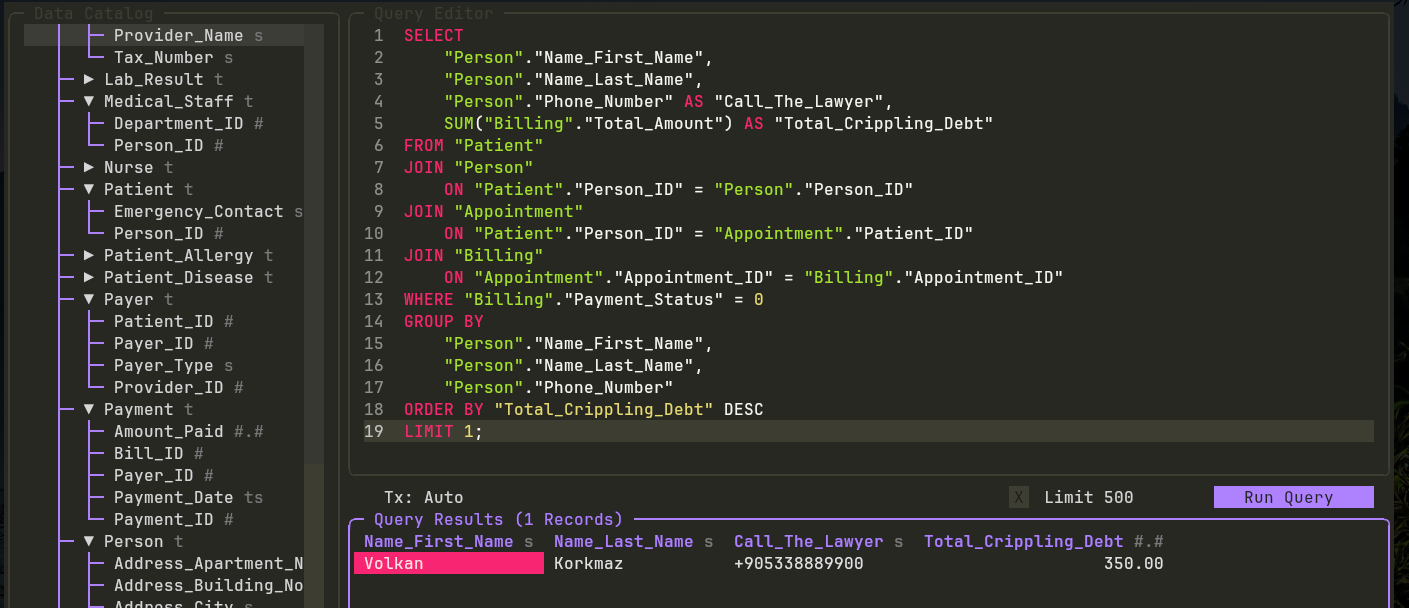
\includegraphics[width=0.8\textwidth]{query_10.png}
	\caption{Patient who owes the most money to the hospital and his number to give to the lawyer}
\end{figure}

\section{Relational Algebra \& Tuple Relational Calculus}
\setcounter{lstlisting}{0}

In this section, the abstract mathematical foundations and logical models of the 5 analytical queries executed in our database architecture are expressed in Relational Algebra (RA) and Tuple Relational Calculus (TRC) formats. The $\gamma$ operator from Extended Relational Algebra was used for grouping and aggregation operations.

\begin{enumerate}

	\item \textbf{Patients with No Appointments} \\
	      \textit{List of patients registered in the system who have not yet scheduled an appointment (Set Difference).}

	      \begin{lstlisting}[language=SQL, caption=Query: Patients with No Appointments, basicstyle=\ttfamily\footnotesize, breaklines=true]
SELECT 
    "Patient"."Person_ID",
    "Person"."Name_First_Name",
    "Person"."Name_Last_Name"
FROM "Patient"
JOIN "Person"
    ON "Patient"."Person_ID" = "Person"."Person_ID"
LEFT JOIN "Appointment"
    ON "Patient"."Person_ID" = "Appointment"."Patient_ID"
WHERE "Appointment"."Appointment_ID" IS NULL;
\end{lstlisting}
	      \begin{itemize}
		      \item \textbf{Relational Algebra:}
		            $$ \begin{aligned} & \pi_{\text{Person\_ID, Name\_First\_Name, Name\_Last\_Name}} ((\text{Patient} \bowtie \text{Person}) \setminus \\ & (\text{Patient} \bowtie \text{Person} \bowtie_{\text{Person\_ID}=\text{Patient\_ID}} \text{Appointment})) \end{aligned} $$
		      \item \textbf{Tuple Relational Calculus:}
		            $$ \begin{aligned} \{ t \mid & \exists p \in \text{Person}, \exists pat \in \text{Patient} \, ( \\ & t.\text{Person\_ID} = pat.\text{Person\_ID} \land t.\text{Name\_First\_Name} = p.\text{Name\_First\_Name} \land \\ & t.\text{Name\_Last\_Name} = p.\text{Name\_Last\_Name} \land pat.\text{Person\_ID} = p.\text{Person\_ID} \land \\ & \neg \exists a \in \text{Appointment} \, (a.\text{Patient\_ID} = pat.\text{Person\_ID})) \} \end{aligned} $$
	      \end{itemize}

	\item \textbf{Patients with Multiple Appointments (COUNT > 1)} \\
	      \textit{Names and total appointment counts of patients who have at least two different appointments.}

	      \begin{lstlisting}[language=SQL, caption=Query: Patients with Multiple Appointments, basicstyle=\ttfamily\footnotesize, breaklines=true]
SELECT 
    "Person"."Name_First_Name",
    "Person"."Name_Last_Name",
    COUNT("Appointment"."Appointment_ID") AS "Total_Appointments"
FROM "Patient"
JOIN "Person"
    ON "Patient"."Person_ID" = "Person"."Person_ID"
JOIN "Appointment"
    ON "Patient"."Person_ID" = "Appointment"."Patient_ID"
GROUP BY 
    "Person"."Name_First_Name",
    "Person"."Name_Last_Name"
HAVING COUNT("Appointment"."Appointment_ID") > 1
ORDER BY "Total_Appointments" DESC;
\end{lstlisting}
	      \begin{itemize}
		      \item \textbf{Relational Algebra:}
		            $$ \begin{aligned} & \pi_{\text{Name\_First\_Name, Name\_Last\_Name}} ( \\ & \sigma_{\text{Total\_App} > 1} (_{\text{Name\_First\_Name, Name\_Last\_Name}} \gamma_{\text{COUNT}(\text{Appointment\_ID}) \to \text{Total\_App}} ( \\ & \text{Patient} \bowtie \text{Person} \bowtie_{\text{Person\_ID}=\text{Patient\_ID}} \text{Appointment}))) \end{aligned} $$
		      \item \textbf{Tuple Relational Calculus (Pure Logical Representation):}
		            $$ \begin{aligned} \{ t \mid & \exists p \in \text{Person}, \exists pat \in \text{Patient}, \exists a_1, a_2 \in \text{Appointment} \, ( \\ & t.\text{Name\_First\_Name} = p.\text{Name\_First\_Name} \land t.\text{Name\_Last\_Name} = p.\text{Name\_Last\_Name} \land \\ & pat.\text{Person\_ID} = p.\text{Person\_ID} \land a_1.\text{Patient\_ID} = pat.\text{Person\_ID} \land \\ & a_2.\text{Patient\_ID} = pat.\text{Person\_ID} \land a_1.\text{Appointment\_ID} \neq a_2.\text{Appointment\_ID}) \} \end{aligned} $$
	      \end{itemize}

	\item \textbf{Corporate Clients (Insurances) Leaderboard} \\
	      \textit{Calculation of total payment amounts generated from insurance-type payers.}

	      \begin{lstlisting}[language=SQL, caption=Query: Corporate Clients Leaderboard, basicstyle=\ttfamily\footnotesize, breaklines=true]
SELECT 
    "Insurance_Provider"."Provider_Name",
    "Insurance_Provider"."Provider_Email",
    SUM("Payment"."Amount_Paid") AS "Total_Corporate_Payment"
FROM "Payer"
JOIN "Insurance_Provider"
    ON "Payer"."Provider_ID" = "Insurance_Provider"."Provider_ID"
JOIN "Payment"
    ON "Payer"."Payer_ID" = "Payment"."Payer_ID"
WHERE "Payer"."Payer_Type" = 'Insurance'
GROUP BY 
    "Insurance_Provider"."Provider_Name",
    "Insurance_Provider"."Provider_Email"
ORDER BY "Total_Corporate_Payment" DESC;
\end{lstlisting}
	      \begin{itemize}
		      \item \textbf{Relational Algebra:}
		            $$ \begin{aligned} & _{\text{Provider\_Name, Provider\_Email}} \gamma_{\text{SUM}(\text{Amount\_Paid}) \to \text{Total\_Corp\_Pay}} ( \\ & \sigma_{\text{Payer\_Type} = \text{'Insurance'}}(\text{Payer}) \bowtie \text{Insurance\_Provider} \bowtie \text{Payment}) \end{aligned} $$
		      \item \textbf{Tuple Relational Calculus:}
		            $$ \begin{aligned} \{ t \mid & \exists ip \in \text{Insurance\_Provider} \, (t.\text{Provider\_Name} = ip.\text{Provider\_Name} \land \\ & t.\text{Provider\_Email} = ip.\text{Provider\_Email} \land t.\text{Total\_Corp\_Pay} = \text{SUM}( \\ & \{ p.\text{Amount\_Paid} \mid \exists py \in \text{Payer} \, (p.\text{Payer\_ID} = py.\text{Payer\_ID} \land \\ & py.\text{Provider\_ID} = ip.\text{Provider\_ID} \land py.\text{Payer\_Type} = \text{'Insurance'}) \} )) \} \end{aligned} $$
	      \end{itemize}

	\item \textbf{Average Billing Amounts by Department} \\
	      \textit{Analysis of average revenue generated by medical departments through appointments.}

	      \begin{lstlisting}[language=SQL, caption=Query: Average Billing Amounts by Department, basicstyle=\ttfamily\footnotesize, breaklines=true]
SELECT 
    "Department"."Department_Name" AS "Disease_Category",
    AVG("Billing"."Total_Amount") AS "Average_Cost"
FROM "Appointment"
JOIN "Doctor"
    ON "Appointment"."Doctor_ID" = "Doctor"."Person_ID"
JOIN "Medical_Staff"
    ON "Doctor"."Person_ID" = "Medical_Staff"."Person_ID"
JOIN "Department"
    ON "Medical_Staff"."Department_ID" = "Department"."Department_ID"
JOIN "Billing"
    ON "Appointment"."Appointment_ID" = "Billing"."Appointment_ID"
GROUP BY "Department"."Department_Name"
ORDER BY "Average_Cost" DESC;
\end{lstlisting}
	      \begin{itemize}
		      \item \textbf{Relational Algebra:}
		            $$ \begin{aligned} & _{\text{Department\_Name}} \gamma_{\text{AVG}(\text{Total\_Amount}) \to \text{Average\_Cost}} ( \\ & \text{Appointment} \bowtie_{\text{Doctor\_ID} = \text{Person\_ID}} \text{Doctor} \bowtie \text{Medical\_Staff} \\ & \bowtie \text{Department} \bowtie \text{Billing}) \end{aligned} $$
		      \item \textbf{Tuple Relational Calculus:}
		            $$ \begin{aligned} \{ t \mid & \exists dep \in \text{Department} \, (t.\text{Disease\_Category} = dep.\text{Department\_Name} \land \\ & t.\text{Average\_Cost} = \text{AVG}( \{ b.\text{Total\_Amount} \mid \exists a \in \text{Appointment}, \\ & \exists doc \in \text{Doctor}, \exists ms \in \text{Medical\_Staff} \, (b.\text{Appointment\_ID} = a.\text{Appointment\_ID} \land \\ & a.\text{Doctor\_ID} = doc.\text{Person\_ID} \land doc.\text{Person\_ID} = ms.\text{Person\_ID} \land \\ & ms.\text{Department\_ID} = dep.\text{Department\_ID}) \} )) \} \end{aligned} $$
	      \end{itemize}

	\item \textbf{Phantom Doctors (Doctors with No Appointments)} \\
	      \textit{Doctors who are registered in the hospital system but have no appointments assigned to them.}

	      \begin{lstlisting}[language=SQL, caption=Query: Doctors with No Appointments, basicstyle=\ttfamily\footnotesize, breaklines=true]
SELECT 
    "Person"."Name_First_Name",
    "Person"."Name_Last_Name"
FROM "Person"
JOIN "Doctor"
    ON "Person"."Person_ID" = "Doctor"."Person_ID"
WHERE NOT EXISTS (
    SELECT 1
    FROM "Appointment"
    WHERE "Appointment"."Doctor_ID" = "Doctor"."Person_ID"
);
\end{lstlisting}
	      \begin{itemize}
		      \item \textbf{Relational Algebra:}
		            $$ \begin{aligned} & \pi_{\text{Name\_First\_Name, Name\_Last\_Name}} ((\text{Person} \bowtie \text{Doctor}) \setminus \\ & (\text{Person} \bowtie \text{Doctor} \bowtie_{\text{Doctor\_ID}=\text{Doctor\_ID}} \text{Appointment})) \end{aligned} $$
		      \item \textbf{Tuple Relational Calculus:}
		            $$ \begin{aligned} \{ t \mid & \exists p \in \text{Person}, \exists d \in \text{Doctor} \, ( \\ & t.\text{Name\_First\_Name} = p.\text{Name\_First\_Name} \land t.\text{Name\_Last\_Name} = p.\text{Name\_Last\_Name} \land \\ & p.\text{Person\_ID} = d.\text{Person\_ID} \land \\ & \neg \exists a \in \text{Appointment} \, (a.\text{Doctor\_ID} = d.\text{Person\_ID})) \} \end{aligned} $$
	      \end{itemize}

\end{enumerate}

\end{document}
